%
% Copyright 2014, General Dynamics C4 Systems
%
% This software may be distributed and modified according to the terms of
% the GNU General Public License version 2. Note that NO WARRANTY is provided.
% See "LICENSE_GPLv2.txt" for details.
%
% @TAG(GD_GPL)
%

\documentclass[a4paper,11pt,twoside]{report}
\usepackage[colour,nictaonly]{disy}

% Setting this to true turns on the `draft' watermark
\newif \ifDraft \Draftfalse

\newif \ifxeightsix   \xeightsixtrue

\usepackage[margin=33mm]{geometry}
\usepackage{graphicx}
\usepackage{cite,url,fancyhdr}

% Draft support
\ifDraft
  \usepackage{draftcopy}
  \newcommand{\Comment}[1]{\textbf{\textsl{#1}}}
  \newcommand{\FIXME}[1]{\textbf{\textsl{FIXME: #1}}}
  \date{}
\else
  \newcommand{\Comment}[1]{\relax}
  \newcommand{\FIXME}[1]{\relax}
  \date{}
\fi

\pagestyle{fancyplain}
\lhead[\fancyplain{}{\sl\thepage}]{\fancyplain{}{\sl\rightmark}}
\chead{}
\rhead[\fancyplain{}{\sl\leftmark}]{\fancyplain{}{\sl\thepage}}
\lfoot[\fancyplain{\sl\thepage}{}]{}
\cfoot{\ifDraft\textsf{NICTA Confidential}\fi}
\rfoot[]{\fancyplain{\sl\thepage}{}}

\usepackage{listings}
\usepackage{multirow}
\usepackage{setspace}
\usepackage{booktabs}
\usepackage{tabularx}
\usepackage{verbatim}
\usepackage[small,bf,up,width=0.75\textwidth]{caption}
\usepackage[htt]{hyphenat}
\renewcommand{\captionfont}{\small}

% Hyperlinks and Colors
\usepackage{color}
%\definecolor{linkcolor}{rgb}{.000,.348,.508}
\definecolor{linkcolor}{rgb}{0, 0, 0}
\usepackage[colorlinks=true,linkcolor=linkcolor,citecolor=linkcolor,
            filecolor=linkcolor,pagecolor=linkcolor,urlcolor=linkcolor]{hyperref}
\renewcommand{\chapterautorefname}{Chapter}
\renewcommand{\sectionautorefname}{Section}
\renewcommand{\subsectionautorefname}{Section}
\renewcommand{\subsubsectionautorefname}{Section}
\renewcommand{\appendixautorefname}{Appendix}
\renewcommand{\Hfootnoteautorefname}{Footnote}
\newcommand{\Htextbf}[1]{\textbf{\hyperpage{#1}}}
\urlstyle{rm}

% API functions / Kernel Objects
\newcommand{\obj}[1]{\textsf{\small #1}}
\newcommand{\apifunc}[2]{\hyperref[api:#2]{\texttt{#1()}}}
\newcommand{\enummem}[1]{\texttt{#1}}
\newcommand{\ipcbloc}[1]{\texttt{#1}}
\newcommand{\reg}[1]{\texttt{#1}}

\newcommand{\version}{\input{VERSION}}

% Read information about the repository.
\input{env}

% Don't indent paragraphs; instead, just leave some vertical space.
\parindent 0pt\parskip 6pt

\begin{document}

  \title{seL4 Reference Manual\\with Asynchronous Endpoint Binding Extensions\\API version \version}

  \author{Trustworthy~Systems~Team, NICTA}
  \AuthorEmail{ssrg@nicta.com.au}
  \date{\commitdate}

  \maketitle

  \urlstyle{sf}
  \thispagestyle{empty}

  \vfill

  \copyright~{\commityear} General Dynamics C4 Systems.\\

  \textsc{All rights reserved}.

  % Acknowledgements
  \thispagestyle{empty}
  \vfill
  \renewcommand{\abstractname}{Acknowledgements}
  \begin{abstract}
% This list of contributors is based on the hg log. If you make commits please
% add your name in alphabetical order.
The primary authors of this document are Matthew Grosvenor and Adam Walker,
with contributions from Adrian Danis, Andrew Boyton, David Greenaway, Etienne
Le Sueur, Gernot Heiser, Gerwin Klein, Godfrey van der Linden, Kevin
Elphinstone, Matthew Fernandez, Matthias Daum, Michael von Tessin, Peter Chubb,
Simon Winwood, Thomas Sewell, Timothy Bourke and Toby Murray. All authors 
and contributors can be contacted at firstname.lastname@nicta.com.au.
  \end{abstract}
  \thispagestyle{empty}

  \cleardoublepage
  \setcounter{page}{1}
  \tableofcontents
  \listoftables
  \listoffigures

  \cleardoublepage
  \setcounter{page}{1}
  \pagenumbering{arabic}

  % Introduction
  %
% Copyright 2014, General Dynamics C4 Systems
%
% This software may be distributed and modified according to the terms of
% the GNU General Public License version 2. Note that NO WARRANTY is provided.
% See "LICENSE_GPLv2.txt" for details.
%
% @TAG(GD_GPL)
%

\chapter{\label{ch:intro}Introduction}

% FIXME: Use of service, mechanism and abstraction is munged through here and the rest of the manual

The seL4 microkernel is an operating-system kernel designed to be
a secure, safe, and reliable foundation for systems in a wide variety of
application domains. As a microkernel, it provides a small number of
services to applications, such as abstractions to create and manage virtual address
spaces, threads, and inter-process communication (IPC). The small number
of services provided by seL4 directly translates to a small
implementation of approximately $8700$ lines of C code. This has allowed
the ARMv6 version of the kernel to be formally proven in the Isabelle/HOL 
theorem prover to adhere to its formal specification~\cite{Boyton_09,Cock_KS_08,Derrin_EKCC_06,Elkaduwe_GE_08,Klein_EHACDEEKNSTW_09,Tuch_KN_07,Winwood_KSACN_09}.

This manual describes the seL4 kernel's API from a user's point of view.
The document starts by giving a brief overview of the seL4 microkernel
design, followed by a reference of the high-level API exposed by the
seL4 kernel to userspace.

While we have tried to ensure that this manual accurately reflects the
behaviour of the seL4 kernel, this document is by no means a formal
specification of the kernel. When the precise behaviour of the kernel
under a particular circumstance needs to be known, users should refer to
the seL4 abstract specification, which
gives a formal description of the seL4 kernel.


  % Chapters
  %
% Copyright 2014, General Dynamics C4 Systems
%
% This software may be distributed and modified according to the terms of
% the GNU General Public License version 2. Note that NO WARRANTY is provided.
% See "LICENSE_GPLv2.txt" for details.
%
% @TAG(GD_GPL)
%

\chapter{\label{ch:objects}Kernel Services and Objects}

A limited number of service primitives are provided by the microkernel;
more complex services may be implemented as applications on top of these
primitives. In this way, the functionality of the system can be extended
without increasing the code and complexity in privileged mode, while
still supporting a potentially wide number of services for varied
application domains.

The basic services seL4 provides are as follows:
\begin{description}
    \item[Threads] are an abstraction of CPU execution that supports
    running software;

    \item[Address spaces] are virtual memory spaces that each contain an
    application. Applications are limited to accessing memory in their
    address space;

    \item[Inter-process communication] (IPC) via \emph{endpoints} allows
    threads to communicate using message passing;

    \item[Notifications] provide a non-blocking signalling mechanism
      similar to binary semaphores;

    \item[Device primitives] allow device drivers to be implemented as
    unprivileged applications.  The kernel exports hardware device
    interrupts via IPC messages; and

    \item[Capability spaces] store capabilities (i.e., access rights) to
    kernel services along with their book-keeping information.
\end{description}

This chapter gives an overview of these services, describes how kernel
objects are accessed by userspace applications, and describes how new
objects can be created.

\section{Capability-based Access Control}
\label{sec:cap-access-control}

The seL4 microkernel provides a capability-based access-control model.
Access control governs all kernel services; in order to perform an
operation, an application must \emph{invoke} a capability in its
possession that has sufficient access rights for the requested service.
With this, the system can be configured to isolate software components from
each other, and also to enable authorised, controlled communication
between components by selectively granting specific communication
capabilities.  This enables software-component isolation with a high
degree of assurance, as only those operations explicitly authorised by
capability possession are permitted.

A capability is an unforgeable token that references a specific kernel
object (such as a thread control block) and carries access rights that
control what methods may be invoked.
Conceptually, a capability resides in an application's \emph{capability
space}; an address in this space refers to a \emph{slot} which may or
may not contain a capability.  An application may refer to
a capability---to request a kernel service, for example---using the
address of the slot holding that capability.  This means, the seL4 
capability model is an instance of a \emph{segregated} (or \emph{partitioned})
capability system, where capabilities are managed by the kernel.

Capability spaces are implemented as a directed graph of kernel-managed
\emph{capability nodes} (\obj{CNode}s).  A \obj{CNode} is a table of
slots, where each slot may contain further \obj{CNode} capabilities. An
address in a capability space is then the concatenation of the indices
of the \obj{CNode} capabilities forming the path to the destination
slot; we discuss \obj{CNode} objects in detail in \autoref{ch:cspace}.

Capabilities can be copied and moved within capability spaces, and
also sent via IPC. This allows creation of applications with specific
access rights, the delegation of authority to another application, and
passing to an application authority to a newly created (or selected)
kernel service. Furthermore, capabilities can be \emph{minted} to
create a derived capability with a subset of the rights of the
original capability (never with more rights). A newly minted
capability can be used for partial delegation of authority.

Capabilities can also be revoked to withdraw
authority. Revocation recursively removes any capabilities that have
been derived from the original capability being revoked. The propagation of
capabilities through the system is controlled by a
\emph{take-grant}-based model~\cite{Elkaduwe_GE_08,Boyton_09}.

\section{System Calls}
\label{sec:syscalls}
\label{sec:sys_send}
\label{sec:sys_wait}
\label{sec:sys_call}
\label{sec:sys_reply}
\label{sec:sys_nbsend}
\label{sec:sys_replywait}
\label{sec:sys_yield}

The seL4 kernel provides a message-passing service for communication between
threads. This mechanism is also used for communication with kernel-provided
services. There is a standard message format, each message containing a
number of data words and possibly some capabilities. The structure and encoding
of these messages are described in detail in \autoref{ch:ipc}. 

Threads send messages by invoking capabilities within their capability space.
When an endpoint capability is invoked in this way, the message will be
transferred through the kernel to another thread. When capabilities to kernel
objects are invoked, the message will be interpreted as a method invocation in a
manner specific to the type of kernel object. For example, invoking a thread
control block (TCB) capability with a correctly formatted message will suspend
the target thread.

Logically, the kernel provides three system calls, \emph{Send},
\emph{Receive} and \emph{Yield}. However, there are also combinations
and variants of the basic \emph{Send} and \emph{Receive} calls, e.g.\
the \emph{Call} operation, which consists of a send followed by a
\emph{Receive} from the same object. Methods on kernel objects other
than endpoints and notifications are all mapped to \emph{Send} or
\emph{Call}, depending on whether or not the method returns a
result. The \emph{Yield} system call is not associated with any kernel
object and is the only operation that does not invoke a capability.

The complete set of system calls is:
\begin{description}
    \item[\apifunc{seL4\_Send}{sel4_send}] delivers a message through the named
    capability and the application to continue. If the invoked
    capability is an endpoint, and no receiver is ready to receive the message
    immediately, the sending thread will block until the message can be
    delivered. No error code or response will be returned by the receiving
    object.

    \item[\apifunc{seL4\_NBSend}{sel4_nbsend}] performs a polling send
      on an endpoint. It
    is similar to \apifunc{seL4\_Send}{sel4_send}, except that it is
    guaranteed not to block. If the message
    cannot be delivered immediately, i.e.\ there is no receiver waiting
    on the destination \obj{Endpoint}, the message is silently dropped. Like
    \apifunc{seL4\_Send}{sel4_send}, no error code or response will be returned.

    \item[\apifunc{seL4\_Call}{sel4_call}] combines \apifunc{seL4\_Send}{sel4_send}
      and \apifunc{seL4\_Wait}{sel4_wait}. The call
      blocks the sending thread until its message is delivered and a reply message is received. When the
    sent message is delivered to another thread (via an
    \obj{Endpoint}), the kernel adds an
    additional `\emph{reply}' capability to the message that is delivered
    to the receiver, giving the latter the right to reply to the original sender. The reply
    capability is deposited in a dedicated slot in the receiver's
    \obj{TCB}, and is a single-use right, meaning that the kernel
    invalidates it as soon as it has been invoked.

    The \apifunc{seL4\_Call}{sel4_call} operation exists not only for
    efficiency reasons (combining two operations into a single system
    call). It differs from
    \apifunc{seL4\_Send}{sel4_send} immediately followed by
    \apifunc{seL4\_Wait}{sel4_wait} in two ways:
    \begin{enumerate}
    \item the single-use reply capability is created to establish a 
      reply channel with minimal trust;
    \item the transition from send to wait phase is atomic, meaning it
      cannot be preempted, and the receiver can reply without any risk
      of blocking.
    \end{enumerate}

    When invoking capabilities to kernel services, using
    \apifunc{seL4\_Call}{sel4_call} allows the kernel to return an error code
    or other response through the reply message.

    \item[\apifunc{seL4\_Wait}{sel4_wait}] is used by a thread to receive
    messages through endpoints or notifications. If no sender or
    notification is pending, the caller
    will block until a message or notification can be delivered. This system call works only on
    \obj{Endpoint} or \obj{Notification} capabilities, raising a fault (see section \ref{sec:faults}) when
    attempted with other capability types.

    \item[\apifunc{seL4\_Reply}{sel4_reply}] is used to respond to a
    \apifunc{seL4\_Call}{sel4_call}, using the reply capability generated by the
    \apifunc{seL4\_Call}{sel4_call} system call and stored in the replying
    thread's TCB. It delivers the message to the thread that invoked
    the \apifunc{seL4\_Call}{sel4_call}, waking it in
    the process.

    There is space for only one reply capability in each thread's TCB, so the
    \apifunc{seL4\_Reply}{sel4_reply} syscall can be used to reply to the most
    recent caller only. The \apifunc{seL4\_CNode\_SaveCaller}{cnode_savecaller}
    method that will be described later can be used to save the reply
    capability into regular capability space, where it can be used with
    \apifunc{seL4\_Send}{sel4_send}.

    \item[\apifunc{seL4\_ReplyWait}{sel4_replywait}] combines \apifunc{seL4\_Reply}{sel4_reply} and
    \apifunc{seL4\_Wait}{sel4_wait}. It exists mostly for efficiency reasons: the common case of
    replying to a request and waiting for the next can be performed in
    a single kernel system call instead of two. The transition from
    the reply to the wait phase is also atomic.

    \item[\apifunc{seL4\_Yield}{sel4_yield}] is the only system call that does not require
    a capability to be used. It forfeits the remainder of the calling thread's
    timeslice and causes invocation of the kernel's scheduler.
    If there are no other runnable threads with the same
    priority as the caller, the calling thread will immediately be
    scheduled with a fresh timeslice.
\end{description}

\section{Kernel Objects}
\label{s:sel4_internals}

In this section we give a brief overview of the kernel-implemented
object types whose instances (also simply called \emph{objects}) can be invoked by applications. The interface to these
objects forms the interface to the kernel itself. The creation and use
of kernel services is achieved by the creation,
manipulation, and combination of these kernel objects:

\begin{description}

    \item[\obj{CNodes}] (see \autoref{ch:cspace}) store capabilities, giving threads permission to
    invoke methods on particular objects.
    Each \obj{CNode} has a fixed number of slots,
    always a power of two, determined when the \obj{CNode} is created. Slots
    can be empty or contain a capability.

    \item[Thread Control Blocks] (\obj{TCB}s; see \autoref{ch:threads}) represent a thread of
    execution in seL4. Threads are the unit of execution that is
    scheduled, blocked, unblocked, etc., depending on the application's
    interaction with other threads.

    \item[\obj{Endpoints}] (see \autoref{ch:ipc}) facilitate message-passing
    communication between threads. IPC is synchronous: A thread
    trying to send or receive on an endpoint blocks until the message
    can be delivered. This means that message delivery only happens if
    a sender and a receiver rendezvous at the endpoint, and the
    kernel can deliver the message with a single copy (or without
    copying for short messages using only registers).

    A capability to an endpoint can be restricted to be
    send-only or receive-only. Additionally, \obj{Endpoint}
    capabilities can have the grant right, which allows sending
    capabilities as part of the message.

    \item[\obj{Notification} Objects] (see \autoref{ch:notifications})
      provide a simple signalling mechanism. A \obj{Notification}
      is a word-size array of flags, each of which behaves like a binary semaphore. Operations
      are \emph{signalling} a subset of flags in a single operation,
      and waiting until any are signalled. Notification capabilities
      can be signal-only or wait-only.

    \item[Virtual Address Space Objects] (see \autoref{ch:vspace}) 
    are used to construct a virtual
    address space (or VSpace) for one or more threads. These
    objects largely directly correspond to those of the hardware, and
    as such are architecture-dependent. The kernel also includes \obj{ASID
    Pool} and \obj{ASID Control} objects for tracking the status of
    address spaces.

    \item[Interrupt Objects] (see \autoref{ch:io}) give applications the ability to receive
    and acknowledge interrupts from hardware devices.
    Initially, there is a capability to \obj{IRQControl},
    which allows for the creation of \obj{IRQHandler} capabilities.
    An \obj{IRQHandler} capability permits the management of a specific 
    interrupt source associated with a specific device.
    It is delegated to
    a device driver to access an interrupt source. The \obj{IRQHandler}
    object allows threads to wait for and acknowledge individual
    interrupts.

    \item[Untyped Memory] (see \autoref{sec:kernmemalloc}) is the foundation of memory allocation
    in the seL4 kernel.  Untyped memory capabilities have a single method
    which allows the creation of new kernel objects. If the method
    succeeds, the calling thread gains access to capabilities to the
    newly-created objects. Additionally, untyped memory objects can be
    divided into a group of smaller untyped memory objects allowing
    delegation of part (or all) of the system's memory.  We discuss
    memory management in general in the following sections.

\end{description}

\section{Kernel Memory Allocation}
\label{sec:kernmemalloc}

The seL4 microkernel does not dynamically allocate memory for kernel objects.
Instead, objects must be explicitly created from application-controlled memory
regions via \obj{Untyped Memory} capabilities.  Applications must have
explicit authority to memory (through these \obj{Untyped Memory} capabilities) in
order to create new objects, and all objects consume a fixed amount of memory once
created. These mechanisms can be used to precisely control
the specific amount of physical memory available to applications,
including being able to enforce isolation of physical memory access
between applications or a device.  There are no arbitrary resource
limits in the kernel apart from those dictated by the
hardware\footnote{The treatment of virtual ASIDs imposes a fixed number
of address spaces. This limitation is to be removed in future
versions of seL4.}, and so many denial-of-service attacks via resource
exhaustion are avoided.

At boot time, seL4 pre-allocates the memory required for the kernel
itself, including the code, data, and stack sections (seL4 is a single
kernel-stack operating system). It then creates an initial user
thread (with an appropriate address and capability space).
The kernel than hands all remaining memory to
the initial thread in the form of capabilities to \obj{Untyped Memory}, and
some additional capabilities to kernel objects that were required to
bootstrap the initial thread.  These \obj{Untyped Memory} regions can then be split into
smaller regions or other kernel objects using the
\apifunc{seL4\_Untyped\_Retype}{untyped_retype} method; the created objects are termed \emph{children} of
the original untyped memory object.

The user-level application that creates an object using \apifunc{seL4\_Untyped\_Retype}{untyped_retype}
receives full authority over the resulting object. It can then delegate
all or part of the authority it possesses over this object to one or
more of its clients.

\subsection{Reusing Memory}
\label{s:memRevoke}

The model described thus far is sufficient for applications to
allocate kernel objects, distribute authority among client
applications, and obtain various kernel services provided by these
objects.  This alone is sufficient for a simple static system
configuration.

The seL4 kernel also allows \obj{Untyped Memory} regions to be reused.
Reusing a region of memory is allowed only
when there are no dangling references (i.e., capabilities) left to the
objects inside that memory.  The kernel tracks
\emph{capability derivations}, i.e., the children generated by the
methods \apifunc{seL4\_Untyped\_Retype}{untyped_retype}, \apifunc{seL4\_CNode\_Mint}{cnode_mint}, \apifunc{seL4\_CNode\_Copy}{cnode_copy}, and
\apifunc{seL4\_CNode\_Mutate}{cnode_mutate}.

The tree structure so generated is termed the \emph{capability
derivation tree} (CDT).\footnote{Although the CDT conceptually is a separate
data structure, it is implemented as part of the CNode object and so
requires no additional kernel meta-data.}  For example, when a user
creates new kernel objects by retyping untyped memory, the newly created
capabilities would be inserted into the CDT as children of the untyped
memory capability.

For each \obj{Untyped Memory} region, the kernel keeps
a \emph{watermark} recording how much of the region has previously been
allocated. Whenever a user requests the kernel to create new objects in
an untyped memory region, the kernel will carry out one of two actions:
if there are already existing objects allocated in the region, the
kernel will allocate the new objects at the current watermark level, and
increase the watermark. If all objects previously allocated in the
region have been deleted, the kernel will reset the watermark and start
allocating new objects from the beginning of the region again.

Finally, the \apifunc{seL4\_CNode\_Revoke}{cnode_revoke} method provided by \obj{CNode} objects
destroys all capabilities derived from the argument capability. Revoking
the last capability to a kernel object triggers the \emph{destroy}
operation on the now unreferenced object. This simply cleans up any in-kernel dependencies between
it, other objects and the kernel.

By calling \apifunc{seL4\_CNode\_Revoke}{cnode_revoke} on the original capability to an untyped memory
object, the user removes all of the untyped memory object's
children---that is, all capabilities pointing to objects in the untyped
memory region.  Thus, after this invocation there are no valid references
to any object within the untyped region, and the region may be safely
retyped and reused.


  %
% Copyright 2014, General Dynamics C4 Systems
%
% This software may be distributed and modified according to the terms of
% the GNU General Public License version 2. Note that NO WARRANTY is provided.
% See "LICENSE_GPLv2.txt" for details.
%
% @TAG(GD_GPL)
%

\chapter{\label{ch:cspace}Capability Spaces}

Recall from \autoref{sec:cap-access-control} that seL4 implements a
capability-based access control model.  Each userspace thread has an
associated \emph{capability space} (CSpace) that contains the
capabilities that the thread possesses, thereby governing which
resources the thread can access.

Recall that capabilities reside within kernel-managed objects known as
\obj{CNode}s. A \obj{CNode} is a table of slots, each of which may
contain a capability. This may include capabilities to further
\obj{CNode}s, forming a directed graph. Conceptually a thread's CSpace
is the portion of the directed graph that is reachable starting with
the \obj{CNode} capability that is its CSpace root.

A CSpace address refers to an individual slot (in
some \obj{CNode} in the CSpace), which may or may not contain a
capability. Threads refer to capabilities in their CSpaces (e.g. when
making system calls) using the address of the slot that holds the
capability in question.  An address in a CSpace is the concatenation
of the indices of the \obj{CNode} capabilities forming the path to the
destination slot; we discuss this further in
\autoref{s:cspace-addressing}.

% FIXME The references to mint in the following paragraph and previously in
% this section need to be cleaned up. They were clearly written at a time when
% it was not possible to change a capability's rights during a CNode_Copy.
Recall that capabilities can be copied and moved within CSpaces, and
also sent in messages (message sending will be described in detail in
\autoref{sec:cap-transfer}).  Furthermore, new capabilities can be
\emph{minted} from old ones with a subset of their rights.  Recall,
from \autoref{s:memRevoke}, that seL4 maintains a \emph{capability
  derivation tree} (CDT) in which it tracks the relationship between
these copied capabilities and the originals.  The revoke method
removes all capabilities (in all CSpaces) that were derived from a
selected capability. This mechanism can be used by servers to restore
sole authority to an object they have made available to clients, or by
managers of untyped memory to destroy the objects in that memory so it
can be retyped.

seL4 requires the programmer to manage all in-kernel data structures,
including CSpaces, from userspace. This means that the userspace
programmer is responsible for constructing CSpaces as well as
addressing capabilities within them.  This chapter first discusses
capability and CSpace management, before discussing how capabilities
are addressed within CSpaces, i.e. how applications can refer to
individual capabilities within their CSpaces when invoking methods.

\section{Capability and CSpace Management}

\subsection{CSpace Creation}

CSpaces are created by creating and manipulating \obj{CNode} objects.
When creating a \obj{CNode} the user must specify the number of slots
that it will have, and this determines the amount of memory that it
will use. Each slot requires 16 bytes of physical memory and has the
capacity to hold exactly one capability. Like any other object, a
\obj{CNode} must be created by calling
\apifunc{seL4\_Untyped\_Retype}{untyped_retype} on an appropriate
amount of untyped memory (see \autoref{sec:object_sizes}).  The caller
must therefore have a capability to enough untyped memory as well as
enough free capability slots available in existing \obj{CNode}s for
the \apifunc{seL4\_Untyped\_Retype}{untyped_retype} invocation to
succeed.

\subsection{CNode Methods}
\label{sec:cnode-ops}

Capabilities are managed largely through invoking \obj{CNode} methods.

\obj{CNodes} support the following methods:
\begin{description}
\item[\apifunc{seL4\_CNode\_Mint}{cnode_mint}] creates a new
  capability in a specified \obj{CNode} slot from an existing
  capability.  The newly created capability may have fewer rights than
  the original and a different guard (see
  \autoref{sec:cap_address_lookup}). \apifunc{seL4\_CNode\_Mint}{cnode_mint}
  can also create a badged capability (see \autoref{sec:ep-badges})
  from an unbadged one.
\item[\apifunc{seL4\_CNode\_Copy}{cnode_copy}] is similar to
  \apifunc{seL4\_CNode\_Mint}{cnode_mint}, but the newly created
  capability has the same badge and guard as the original.
\item[\apifunc{seL4\_CNode\_Move}{cnode_move}] moves a capability
  between two specified capability slots. You cannot move a capability
  to the slot in which it is currently.
\item[\apifunc{seL4\_CNode\_Mutate}{cnode_mutate}] can move a
  capability similarly to \apifunc{seL4\_CNode\_Move}{cnode_move} and
  also reduce its rights similarly to
  \apifunc{seL4\_CNode\_Mint}{cnode_mint}, although without an
  original copy remaining.
\item[\apifunc{seL4\_CNode\_Rotate}{cnode_rotate}] moves two
  capabilities between three specified capability slots. It is
  essentially two \apifunc{seL4\_CNode\_Move}{cnode_move} invocations:
  one from the second specified slot to the first, and one from the
  third to the second. The first and third specified slots may be the
  same, in which case the capability in it is swapped with the
  capability in the second slot. The method is atomic; either both or
  neither capabilities are moved.
\item[\apifunc{seL4\_CNode\_Delete}{cnode_delete}] removes a
  capability from the specified slot.
\item[\apifunc{seL4\_CNode\_Revoke}{cnode_revoke}] is equivalent to
  calling \apifunc{seL4\_CNode\_Delete}{cnode_delete} on each derived
  child of the specified capability. It has no effect on the
  capability itself, except in very specific circumstances outlined
  in Section~\ref{s:cspace-revoke}.
\item[\apifunc{seL4\_CNode\_SaveCaller}{cnode_savecaller}] moves a
  kernel-generated reply capability of the current thread from the
  special \obj{TCB} slot it was created in, into the designated CSpace
  slot.
\item[\apifunc{seL4\_CNode\_CancelBadgedSends}{cnode_cancelbadgedsends}] cancels
  any outstanding sends that use the same badge and object as the
  specified capability.
\end{description}

\subsection{Capabilities to Newly-Retyped Objects}
\label{sec:caps_to_new_objects}

When retyping untyped memory into objects with
\apifunc{seL4\_Untyped\_Retype}{untyped_retype}, capabilities to the
newly-retyped objects are placed in consecutive slots in a
\obj{CNode} specified by its \texttt{root}, \texttt{node\_index}, and
\texttt{node\_depth} arguments. The \texttt{node\_offset} argument specifies the
index into the \obj{CNode} at which the first capability will be placed.
The \texttt{num\_objects} argument specifies the number of capabilities (and, hence, objects)
to create. All slots must be empty or an error will result. All resulting
capabilities will be placed in the same \obj{CNode}.

\subsection{Capability Rights}
\label{sec:cap_rights}

As mentioned previously, some capability types have \emph{access
  rights} associated with them. Currently, access rights are
associated with capabilities for \obj{Endpoint}s (see
\autoref{ch:ipc}), \obj{Notification}s (see
\autoref{ch:notifications}) and \obj{Page}s (see \autoref{ch:vspace}).  The
access rights associated with a capability determine the methods that
can be invoked.  seL4 supports three orthogonal access rights, which
are Read, Write and Grant.  The meaning of each right is interpreted
relative to the various object types, as detailed
in~\autoref{tab:rights}.

When an object is first created, the initial capability that refers to
it carries the maximum set of access rights. Other, less-powerful
capabilities may be manufactured from this original capability, using
methods such as \apifunc{seL4\_CNode\_Mint}{cnode_mint} and
\apifunc{seL4\_CNode\_Mutate}{cnode_mutate}.  If a greater set of
rights than the source capability is specified for the destination
capability in either of these invocations, the destination rights are
silently downgraded to those of the source.

\begin{table}[htb]
  \begin{tabularx}{\textwidth}{p{0.15\textwidth}XXX}
    \toprule
    Type & Read & Write & Grant \\
    \midrule
    \obj{Endpoint} & Required to receive. & Required to send. & Required to send capabilities (including reply capabilities).\\
    \obj{Notification} & Required to wait. & Required to signal. & N/A \\
    \obj{Page} & Required to map the page readable. & Required to map the page writable. & N/A \\
    \bottomrule
  \end{tabularx}
  \caption{\label{tab:rights}seL4 access rights.}
\end{table}

\subsection{Capability Derivation Tree}
\label{sec:cap_derivation}

As mentioned in \autoref{s:memRevoke}, seL4 keeps track of capability
derivations in a capability derivation tree.

Various methods, such as \apifunc{seL4\_CNode\_Copy}{cnode_copy} or
\apifunc{seL4\_CNode\_Mint}{cnode_mint}, may be used to create derived
capabilities. Not all capabilities support derivation. In general,
only \emph{original} capabilities support derivation invocations, but
there are exceptions.  \autoref{tab:cap-derivation} summarises the
conditions that must be met for capability derivation to succeed for
the various capability types, and how capability-derivation failures
are reported in each case. The capability types not listed can be
derived once.

\begin{table}[htb]
  \begin{tabularx}{\textwidth}{p{0.25\textwidth}XX}
    \toprule
    Cap Type & Conditions for Derivation & Error Code on Derivation Failure \\
    \midrule
    \obj{ReplyCap} & Cannot be derived & Dependent on syscall \\
    \obj{IRQControl} & Cannot be derived & Dependent on syscall \\
    \obj{Untyped} & Must not have children (\autoref{s:cspace-revoke}) & \enummem{seL4\_RevokeFirst} \\
    \obj{Page Table} & Must be mapped & \enummem{seL4\_IllegalOperation} \\
    \obj{Page Directory} & Must be mapped & \enummem{seL4\_IllegalOperation}\\
    \ifxeightsix
    \obj{IO Page Table (IA-32 only)} & Must be mapped & \enummem{seL4\_IllegalOperation}\\
    \fi \bottomrule
  \end{tabularx}
  \caption{Capability derivation.\label{tab:cap-derivation}}
\end{table}

\begin{figure}[th]
  \begin{center}
    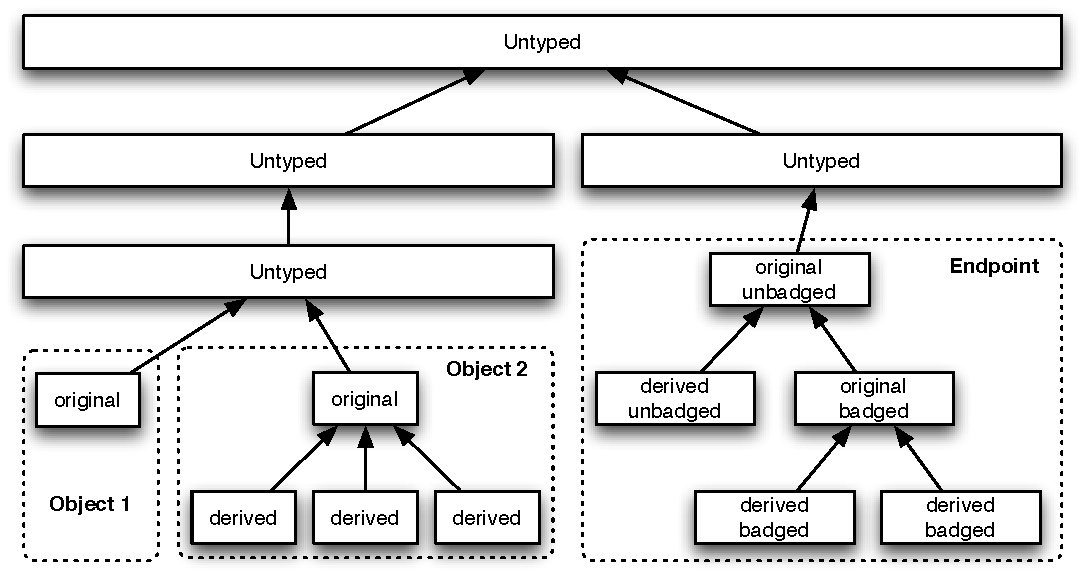
\includegraphics[width=0.8\textwidth]{figs/CDT}
  \end{center}
  \caption{Example capability derivation tree.}\label{fig:CDT}
\end{figure}

\autoref{fig:CDT} shows an example capability derivation tree that
illustrates a standard scenario: the top level is a large untyped
capability, the second level splits this capability into two regions
covered by their own untyped caps, both are children of the first
level.  The third level on the left is a copy of the level 2 untyped
capability.  Untyped capabilities when copied always create children,
never siblings.  In this scenario, the untyped capability was typed
into two separate objects, creating two capabilities on level 4, both
are the original capability to the respective object, both are
children of the untyped capability they were created from.

Ordinary original capabilities can have one level of derived
capabilities.  Further copies of these derived capabilities will
create siblings, in this case remaining on level 5. There is an
exception to this scheme for \obj{Endpoint} and \obj{Notification} capabilities --- they support an
additional layer of depth though \emph{badging}.
The original \obj{Endpoint} or \emph{Notification} capability will be unbadged. Using
the mint method, a copy of the capability with a specific \emph{badge} can be
created (see \autoref{s:ep-badge}, \autoref{s:notif-badge}). This new, badged capability to the same object is treated as
an original capability (the ``original badged endpoint capability'')
and supports one level of derived children like other capabilities.


\section{Deletion and Revocation}
\label{s:cspace-revoke}

Capabilities in seL4 can be deleted and revoked. Both methods
primarily affect capabilities, but they can have side effects on
objects in the system where the deletion or revocation results in the
destruction of the last capability to an object.

As described above, \apifunc{seL4\_CNode\_Delete}{cnode_delete} will
remove a capability from the specified CNode slot. Usually, this is
all that happens. If, however, it was the last typed capability to an
object, this object will now be destroyed by the kernel, cleaning up
all remaining in-kernel references and preparing the memory for
re-use.

If the object to be destroyed was a capability container, i.e.\ a TCB
or CNode, the destruction process will delete each capability held in
the container, prior to destroying the container. This may result in
the destruction of further objects if the contained capabilities are
the last capabilities.\footnote{The recursion is limited as if the last
capability to a CNode is found within the container, the found CNode
is not destroyed. Instead, the found CNode is made unreachable by
moving the capability pointing to the found CNode into the found cnode
itself, by swapping the capability with the first capability in the
found cnode, and then trying to delete the swapped capability
instead. This breaks the recursion.

The result of this approach is that deleting the last cap to the root
CNode of a CSpace does not recursively delete the entire
CSpace. Instead, it deletes the root CNode, and the branches of the
tree become unreachable, potentially including the deleting of some of
the unreachable CNode's caps to make space for the self-referring
capability. The practical consequence of this approach is that CSpace
deletion requires user-level to delete the tree leaf first if
unreachable CNodes are to be avoided. Alternatively, any resulting
unreachable CNodes can be cleaned up via revoking a covering untyped
capability, however this latter approach may be more complex to
arrange by construction at user-level.}

The \apifunc{seL4\_CNode\_Revoke}{cnode_revoke} method will
\apifunc{seL4\_CNode\_Delete}{cnode_delete} all CDT children of the
specified capability, but will leave the capability itself intact. If
any of the revoked child capabilities were the last capabilities to an
object, the appropriate destroy operation is triggered.

Note: \apifunc{seL4\_CNode\_Revoke}{cnode_revoke} may only partially
complete in two specific circumstances. The first being where a
CNode containing the last capability to the TCB of the thread
performing the revoke (or the last capability to the TCB itself) is
deleted as a result of the revoke. In this case the thread performing
the revoke is destroyed during the revoke and the revoke does not
complete. The second circumstance is where the storage containing the
capability that is the target of the revoke is deleted as a result of
the revoke. In this case, the authority to perform the revoke is
removed during the operation and the operation stops part way
through. Both these scenarios can be and should be avoided at
user-level by construction.

Note that for page tables and page directories
\apifunc{seL4\_CNode\_Revoke}{cnode_revoke} will not revoke frame
capabilities mapped into the address space.  They will only be
unmapped from the space.


\section{CSpace Addressing}
\label{s:cspace-addressing}

When performing a system call, a thread specifies to the kernel the
capability to be invoked by giving an address in its CSpace. This
address refers to the specific slot in the caller's CSpace that
contains the capability to be invoked.

CSpaces are designed to permit sparsity, and the process of looking-up
a capability address must be efficient. Therefore, CSpaces are
implemented as \emph{guarded page tables}.
% FIXME: need a references to justify the above decision

As explained earlier, a CSpace is a directed graph of \obj{CNode}
objects, and each \obj{CNode} is a table of slots, where each slot can
either be empty, or contain a capability, which may refer to another \obj{CNode}.
Recall from \autoref{s:sel4_internals} that the number of slots in a \obj{CNode}
must be a power of two. A \obj{CNode} is said to have a \emph{radix}, which is
the power to which two is raised in its size. That is, if a \obj{CNode} has
$2^k$ slots, its radix would be $k$.
The kernel stores a capability to the root \obj{CNode} of each thread's
CSpace in the thread's TCB. Conceptually, a \obj{CNode} capability
stores not only a reference to the \obj{CNode} to which it refers, but
also carries a \emph{guard} value, explained in
\autoref{sec:cap_address_lookup}.

\subsection{Capability Address Lookup}
\label{sec:cap_address_lookup}
Like a virtual memory address, a capability address is simply an
integer. Rather than referring to a location of physical memory (as
does a virtual memory address), a capability address refers to a
capability slot.  When looking up a capability address presented by a
userspace thread, the kernel first consults the \obj{CNode} capability
in the thread's TCB that defines the root of the thread's CSpace. It
then compares that \obj{CNode}'s \emph{guard} value against the most
significant bits of the capability address.  If the two values are
different, lookup fails. Otherwise, the kernel then uses the next
most-significant \emph{radix} bits of the capability address as an
index into the \obj{CNode} to which the \obj{CNode} capability
refers. The slot~$s$ identified by these next \emph{radix} bits might
contain another \obj{CNode} capability or contain something else
(including nothing).  If $s$ contains a \obj{CNode} capability~$c$ and
there are remaining bits (following the \emph{radix} bits) in the
capability address that have yet to be translated, the lookup process
repeats, starting from the \obj{CNode} capability~$c$ and using these
remaining bits of the capability address. Otherwise, the lookup
process terminates successfully; the capability address in question
refers to the capability slot~$s$.

\begin{figure}[tb]
    \begin{center}
        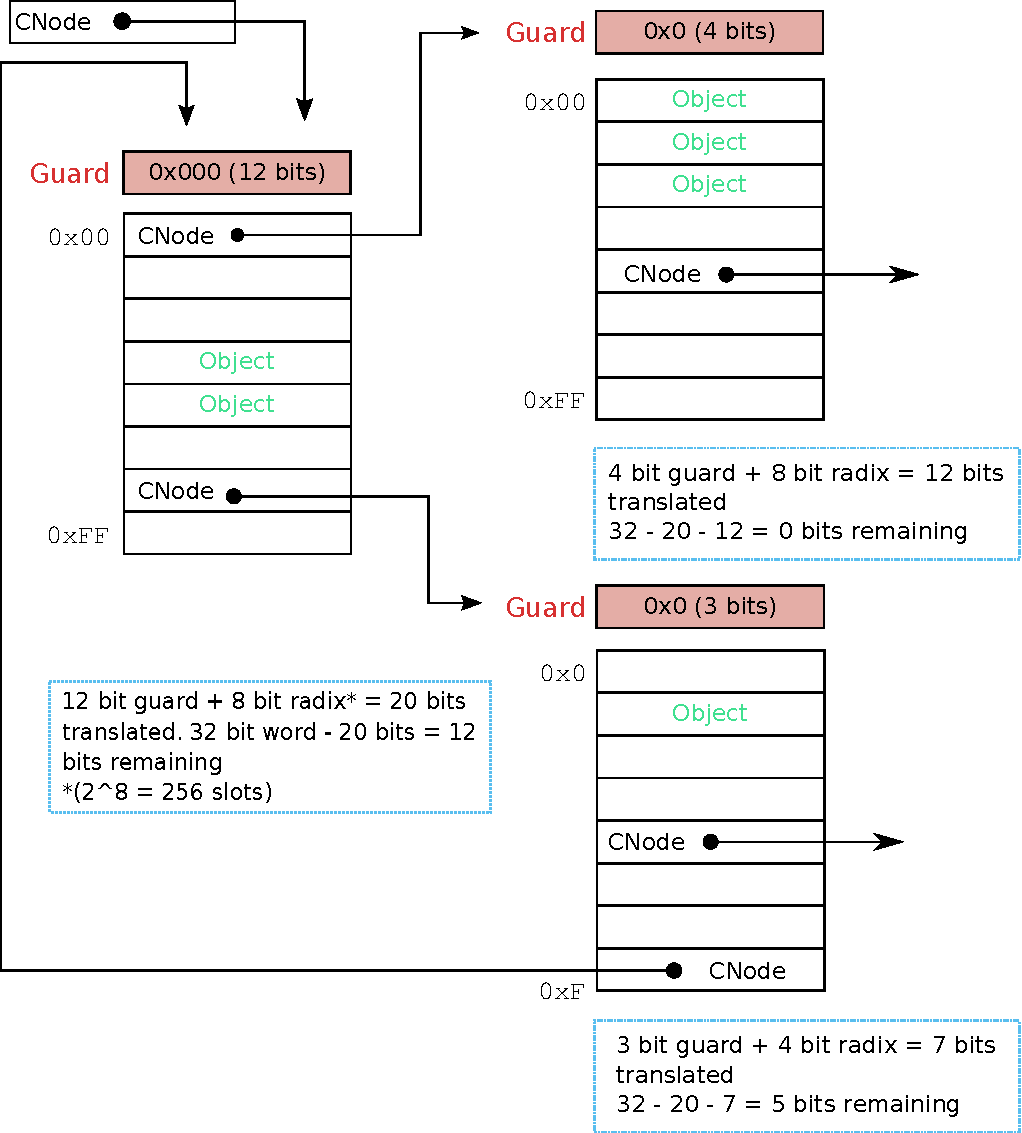
\includegraphics[scale=0.5]{figs/fig1-4.pdf}
        \caption{An example CSpace demonstrating object references at
          all levels, various guard and radix sizes and internal CNode
          references.}
        \label{fig1.4}
    \end{center}
\end{figure}

Figure \ref{fig1.4} demonstrates a valid CSpace with the following
features:
\begin{itemize}
\item a top level CNode object with a 12-bit guard set to 0x000 and
  256 slots;
\item a top level CNode with direct object references;
\item a top level CNode with two second-level CNode references;
\item second level CNodes with different guards and slot counts;
\item a second level CNode that contains a reference to a top level
  CNode;
\item a second level CNode that contains a reference to another CNode
  where there are some bits remaining to be translated;
\item a second level CNode that contains a reference to another CNode
  where there are no bits remaining to be translated; and
\item object references in the second level CNodes.
\end{itemize}

It should be noted that \autoref{fig1.4} demonstrates only what is
possible, not what is usually practical. Although the CSpace is legal,
it would be reasonably difficult to work with due to the small number
of slots and the circular references within it.


\subsection{Addressing Capabilities}
\label{sec:cap_addressing}

A capability address is stored in a CPointer (abbreviated CPTR), which
is an unsigned integer variable. Capabilities are addressed in
accordance with the translation algorithm described above.  Two
special cases involve addressing \obj{CNode} capabilities themselves
and addressing a range of capability slots.

Recall that the translation algorithm described above will traverse
\obj{CNode} capabilities while there are address bits remaining to be
translated. Therefore, in order to address a \obj{CNode} capability,
the user must supply not only a capability address but also specify
the maximum number of bits of the capability address that are to be
translated, called the \emph{depth limit}.

Certain methods, such as
\apifunc{seL4\_Untyped\_Retype}{untyped_retype}, require the user to
provide a range of capability slots. This is done by providing a base
capability address, which refers to the first slot in the range,
together with a window size parameter, specifying the number of slots
(with consecutive addresses, following the base slot) in the range.


\autoref{fig2.1} depicts an example CSpace. In order to illustrate
these ideas, we determine the address of each of the 10 capabilities
in this CSpace.

\begin{figure}[tb]
  \begin{center}
    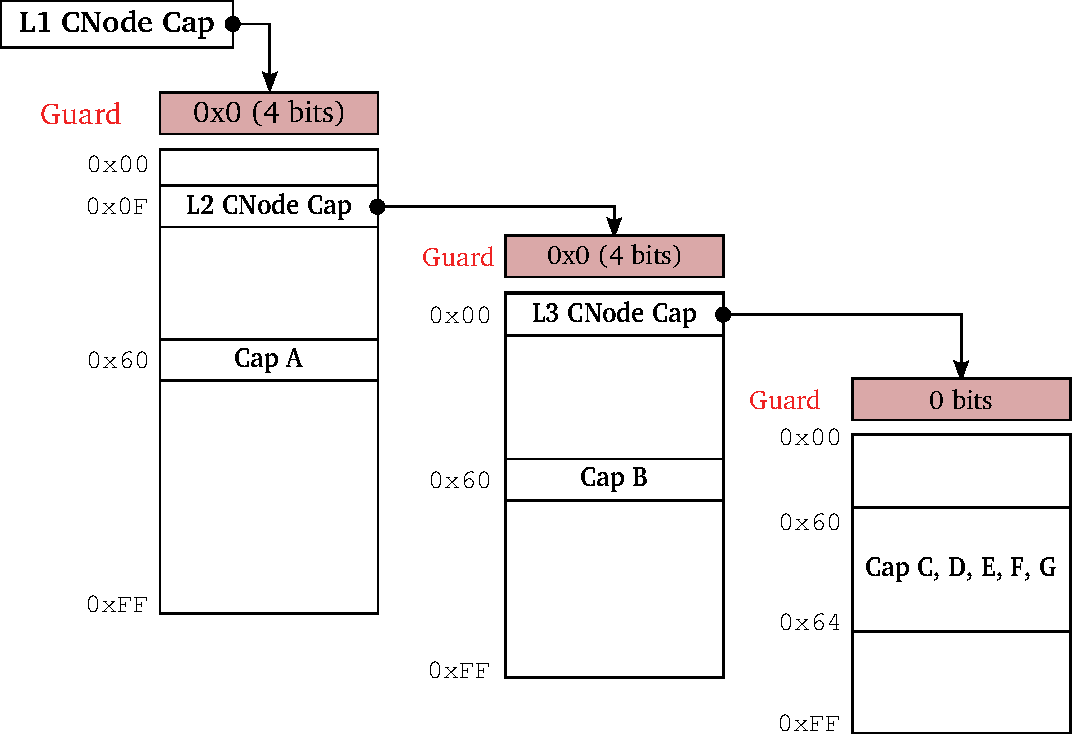
\includegraphics[scale=0.5]{figs/fig2-1.pdf}
    \caption{An arbitrary CSpace layout.}
    \label{fig2.1}
  \end{center}
\end{figure}


\begin{description}
\item[Cap A.] The first CNode has a 4-bit guard set to 0x0, and an
  8-bit radix. Cap A resides in slot 0x60 so it may be referred to by
  any address of the form 0x060xxxxx (where xxxxx is any number,
  because the translation process terminates after translating the
  first 12 bits of the address). For simplicity, we usually adopt the
  address 0x06000000.

\item[Cap B.] Again, the first CNode has a 4-bit guard set to 0x0, and
  an 8-bit radix. The second CNode is reached via the L2 CNode Cap.
  It also has a 4-bit guard of 0x0 and Cap B resides at index
  0x60. Hence, Cap B's address is 0x00F06000.  Translation of this
  address terminates after the first 24 bits.

\item[Cap C.] This capability is addressed via both CNodes. The third
  CNode is reached via the L3 CNode Cap, which resides at index 0x00
  of the second CNode. The third CNode has no guard and Cap C is at
  index 0x60.  Hence, its address is 0x00F00060. Translation of this
  address leaves 0 bits untranslated.

\item[Caps C--G.] This range of capability slots is addressed by
  providing a base address (which refers to the slot containing Cap C)
  of 0x00F00060 and a window size of 5.

\item[L2 CNode Cap.] Recall that to address a \obj{CNode} capability,
  the user must supply not only a capability address but also specify
  the depth limit, which is the maximum number of bits to be
  translated.  L2 CNode Cap resides at offset 0x0F of the first CNode,
  which has a 4-bit guard of 0x0.  Hence, its address is 0x00F00000,
  with a depth limit of 12 bits.

\item[L3 CNode Cap.] This capability resides at index 0x00 of the
  second CNode, which is reached by the L2 CNode Cap. The second CNode
  has a 4-bit guard of 0x0. Hence, the capability's address is
  0x00F00000 with a depth limit of 24 bits. Note that the addresses of
  the L2 and L3 CNode Caps are the same, but that their depth limits
  are different.
\end{description}

In summary, to refer to any capability (or slot) in a CSpace, the user
must supply its address. When the capability might be a CNode, the
user must also supply a depth limit.  To specify a range of capability
slots, the user supplies a starting address and a window size.

\section{Lookup Failure Description}
\label{sec:lookup_fail_desc}

When a capability lookup fails, a description of the failure is given
to either the calling thread or the thread's exception handler in its
IPC buffer.  The format of the description is always the same but may
occur at varying offsets in the IPC buffer depending on how the error
occurred.  The description format is explained below.  The first word
indicates the type of lookup failure and the meaning of later words
depend on this.

\subsection{Invalid Root}

A CSpace CPTR root (within which a capability was to be looked up)
is invalid. For example, the capability is not a \obj{CNode} cap.\\  \\

\begin{tabularx}{\textwidth}{XX}
  \toprule
  Data & Meaning \\
  \midrule
  \ipcbloc{Offset + 0} & \enummem{seL4\_InvalidRoot} \\
  \bottomrule
\end{tabularx}

\subsection{Missing Capability}

A capability required for an invocation is not present or does not
have sufficient rights. \\ \\

\begin{tabularx}{\textwidth}{XX}
  \toprule
  Data & Meaning \\
  \midrule
  \ipcbloc{Offset + 0} & \enummem{seL4\_MissingCapability} \\
    \ipcbloc{Offset + seL4\_CapFault\_BitsLeft} & Bits left \\
  \bottomrule
\end{tabularx}

\subsection{Depth Mismatch}

When resolving a capability, a CNode was traversed that resolved more
bits than was left to decode in the CPTR or a non-CNode capability was
encountered while there were still bits remaining to be looked up. \\ \\

\begin{tabularx}{\textwidth}{XX}
  \toprule
  Data & Meaning \\
  \midrule
  \ipcbloc{Offset + 0} & \enummem{seL4\_DepthMismatch} \\
  \ipcbloc{Offset + seL4\_CapFault\_BitsLeft} & Bits of CPTR remaining to decode \\
  \ipcbloc{Offset + seL4\_CapFault\_DepthMismatch\_BitsFound} & Bits that the current CNode being traversed resolved \\
  \bottomrule
\end{tabularx}

\subsection{Guard Mismatch}

When resolving a capability, a CNode was traversed with a guard size
larger than the number of bits remaining or the CNode's guard did not
match the next bits of the CPTR being resolved. \\ \\

\begin{tabularx}{\textwidth}{XX}
  \toprule
  Data & Meaning \\
  \midrule
  \ipcbloc{Offset + 0} & \enummem{seL4\_GuardMismatch} \\
    \ipcbloc{Offset + seL4\_CapFault\_BitsLeft} & Bits of CPTR remaining to decode \\
  \ipcbloc{Offset + seL4\_CapFault\_GuardMismatch\_GuardFound} & The CNode's guard \\
  \ipcbloc{Offset + seL4\_CapFault\_GuardMismatch\_BitsFound} & The CNode's guard size \\
  \bottomrule
\end{tabularx}



  %
% Copyright 2014, General Dynamics C4 Systems
%
% This software may be distributed and modified according to the terms of
% the GNU General Public License version 2. Note that NO WARRANTY is provided.
% See "LICENSE_GPLv2.txt" for details.
%
% @TAG(GD_GPL)
%

\chapter{\label{ch:ipc}Inter-process Communication}

The seL4 microkernel provides a message-passing mechanism for communication
between threads. The mechanism is also used for communication with
kernel-provided services. Messages are sent by invoking a capability to a
kernel object. Messages sent to \emph{synchronous} (\obj{Endpoint}) and
\emph{asynchronous} (\obj{Async\-EP}) IPC endpoints are destined for other
threads; messages sent to objects of other types are processed by the kernel. This
chapter describes the common message format, the two types of endpoints,
and how they can be used for communication between applications.

\section{Message Registers}
\label{sec:messageinfo}

Each message contains a number of message words and optionally a number of
capabilities.
The message words are sent to or received from a thread by placing them in its \emph{message registers}.
The message registers are numbered and the first few message registers are implemented
using physical CPU registers, while the rest are backed by a fixed region of
memory called the \emph{IPC buffer}.
The reason for this design is efficiency:
very short messages need not use the memory.
The physical CPU registers used for the
message registers are described in \ifxeightsix\autoref{tbl:mrs_x86} for x86
% x86 is used rather than IA-32 to be vendor neutral.
and \fi \autoref{tbl:mrs_arm} for ARM.
The IPC buffer is assigned to the calling thread (see \autoref{sec:threads} and \autoref{api:tcb_setipcbuffer}).
%FIXME: seL4_TCB_SetIPCBuffer is only mentioned in the API reference!

\ifxeightsix
\begin{table}[htb]
    \begin{center}
        \begin{tabular}{lc}
            \toprule
            Role                                    & CPU Register \\
            \midrule
            Capability register \emph{(in)}         & \texttt{ebx} \\
            Badge register \emph{(out)}             & \texttt{ebx} \\
            Message tag \emph{(in/out)}     & \texttt{esi} \\
            Message register 1 \emph{(in/out)}      & \texttt{edi} \\
            Message register 2 \emph{(in/out)}      & \texttt{ebp} \\
            \bottomrule
        \end{tabular}
    \caption{\label{tbl:mrs_x86}Physical register allocation for IPC messages
    on the x86 architecture.}
    \end{center}
\end{table}
\fi

\begin{table}[htb]
    \begin{center}
        \begin{tabular}{lc}
            \toprule
            Role                                    & CPU Register \\
            \midrule
            Capability register \emph{(in)}         & \texttt{r0} \\
            Badge register \emph{(out)}             & \texttt{r0} \\
            Message tag \emph{(in/out)}     & \texttt{r1} \\
            Message register 1--4 \emph{(in/out)}   & \texttt{r2} -- \texttt{r5} \\
            \bottomrule
        \end{tabular}
    \caption{\label{tbl:mrs_arm}Physical register allocation for IPC messages on the ARM architecture.}
    \end{center}
\end{table}

Every IPC message also has a tag (structure \texttt{seL4\_MessageInfo\_t}).  The
tag consists of four fields: the label, message length, number of capabilities
(the \texttt{extraCaps} field) and the \texttt{capsUnwrapped} field.  The
message length and number of capabilities determine either the number of
message registers and capabilities that the sending thread wishes to transfer,
or the number of message registers and capabilities that were actually
transferred. The label is not interpreted by the
kernel and is passed unmodified as the first data payload of the message. The
label may, for example, be used to specify a requested operation. The
\texttt{capsUnwrapped} field is used only on the receive side, to indicate the
manner in which capabilities were received. It is described in
\autoref{sec:cap-transfer}.

% FIXME: a little too low-level, perhaps?

\newcommand{\ipcparam}[4]{\texttt{#1} \emph{#2}&\texttt{#3}&#4\\ }
\begin{table}[htb]
    \begin{center}
    \begin{tabularx}{\textwidth}{p{0.28\textwidth}p{0.18\textwidth}X}
      \toprule
      \textbf{Type} & \textbf{Name} & \textbf{Description} \\
      \midrule
        \ipcparam{seL4\_MessageInfo\_t}{}{tag}{Message tag}
        \ipcparam{seL4\_Word[]}{}{msg}{Message contents}
        \ipcparam{seL4\_Word}{}{userData}{Base address of the structure, used by
        supporting user libraries}
        \ipcparam{seL4\_CPtr[]}{(in)}{caps}{Capabilities to transfer}
        \ipcparam{seL4\_CapData\_t[]}{(out)}{badges}{Badges for
        endpoint capabilities received}
        \ipcparam{seL4\_CPtr}{}{receiveCNode}{CPTR to a CNode from which to
        find
        the receive slot}
        \ipcparam{seL4\_CPtr}{}{receiveIndex}{CPTR to the receive slot
        relative to \texttt{receiveCNode}}
        \ipcparam{seL4\_Word}{}{receiveDepth}{Number of bits of
        \texttt{receiveIndex} to
        use}
        \bottomrule
      \end{tabularx}
    \caption{\label{tbl:ipcbuffer}Fields of the
      \texttt{seL4\_IPCBuffer} structure.  Note that
      \texttt{badges} and \texttt{caps} use the same area of memory in
      the structure.}
    \end{center}
\end{table}

The kernel assumes that the IPC buffer contains a structure of type
\texttt{seL4\_IPCBuffer} as defined in \autoref{tbl:ipcbuffer}. The
kernel uses as many physical registers as possible to transfer IPC
messages. When more arguments are transferred than physical message
registers are available, the kernel begins using the IPC buffer's
\texttt{msg} field to transfer arguments. However, it leaves room in
this array for the physical message registers. For example, if an IPC
transfer or kernel object invocation required
4 message registers (and there are only 2 physical message registers
available on this architecture) then arguments 1 and 2 would be
transferred via message registers and arguments 3 and 4 would be in
\texttt{msg[2]} and \texttt{msg[3]}.
This allows the user-level object-invocation stubs to copy the arguments passed in physical registers to
the space left in the \texttt{msg} array if desired.
The situation is similar for the tag field.
There is space for this field in the \texttt{seL4\_IPCBuffer} structure, which the kernel ignores.
User level stubs
may wish to copy the message tag from its CPU register to this field, although
the user level stubs provided with the kernel do not do this.

\section{Synchronous Endpoints}

Synchronous endpoints (or simply \obj{Endpoint}s) allow a small amount
of data and small number of capabilities (namely the IPC buffer) to be transferred between two
threads. \obj{Endpoints} are called
`synchronous' because a message transfer will not take
place until both the sender is ready to send the message and a receiver is
ready to receive it.

\obj{Endpoint} objects are invoked directly using the seL4 system calls
described in \autoref{sec:syscalls}. Note that \obj{Endpoint} objects may queue
threads either to send or to receive. If no receiver is ready, threads
performing the \apifunc{seL4\_Send}{sel4_send} or \apifunc{seL4\_Call}{sel4_call}
system calls will wait in a queue for the first available receiver. Likewise if
no sender is ready, threads performing the \apifunc{seL4\_Wait}{sel4_wait}
system call or the second half of \apifunc{seL4\_ReplyWait}{sel4_replywait}
will wait for the first available sender.

\subsection{Endpoint Badges}
\label{sec:ep-badges}

Synchronous endpoint capabilities may be \emph{minted} to
create a new endpoint capability with a \emph{badge} attached to it. The
badge is a word of data that is associated with a particular endpoint
capability. When a message is sent to an endpoint using a badged
capability, the badge is transferred to the receiving thread's
\texttt{badge} register.

An endpoint capability with a zero badge is said to be \emph{unbadged}.
Such a capability can be badged with the \apifunc{seL4\_CNode\_Mutate}{cnode_mutate} or \apifunc{seL4\_CNode\_Mint}{cnode_mint}
invocations on the \obj{CNode} containing the capability. Endpoint
capabilities with badges cannot be unbadged, rebadged or used to create
child capabilities with different badges.

\subsection{Capability Transfer}
\label{sec:cap-transfer}

Messages in seL4 may contain capabilities. Messages containing capabilities can
be sent across synchronous endpoints, provided that the endpoint capability
invoked by the sending thread has Grant rights. An attempt to transfer
capabilities without Grant rights can still result in the message being sent,
but no capabilities will be transferred.

Capabilities to be sent with a message are specified in the sending thread's
IPC buffer in the \texttt{caps} field. Each entry in that array is interpreted
as a CPTR in the sending thread's capability space. The number of capabilities
to send is specified in the \texttt{extraCaps} field of the message tag.

The receiver specifies the slot,
in which it is willing to receive a capability, with three fields within the IPC buffer: \texttt{receiveCNode}, \texttt{receiveIndex} and \texttt{receiveDepth}.
These fields specify the root CNode, capability address and number of bits to resolve, respectively, to find
the slot in which to put the capability. Capability
addressing is described in \autoref{sec:cap_addressing}.

A received capability has the same rights as the original except if the receiving endpoint capability does not have the Write right.
In this case, the rights on the sent capability are \emph{diminished}, by
removing from the received copy of that capability the Write right.

Note that receiving threads may specify only one receive slot, whereas a
sending thread may include multiple capabilities in the message. Messages
containing more than one capability may be interpreted by kernel objects. They
may also be sent to receiving threads in the case where some of the extra
capabilities in the message can be \emph{unwrapped}.

If the n-th capability in the message refers to the same endpoint as the one
the
message is being sent through, it is \emph{unwrapped}. Its badge is placed in
the n-th
position of the receiver's badges array and the n-th bit (counting from the
least significant) is set in the \texttt{capsUnwrapped} field of the message
tag. The capability itself is not transferred, so the receive slot may be used
for another one.

If a receiver gets a message whose tag has an \texttt{extraCaps} of 2 and a
\texttt{capsUnwrapped} of 2, then the first capability in the message was
transferred to the specified receive slot and the second capability was
unwrapped, placing its badge in \texttt{badges[1]}. There may have been a
third capability in the sender's message which could not be unwrapped.

\subsection{Errors}

% FIXME : will this actually issue a fault? TS: in the send phase? yes, yes it will

Errors in capability transfers can occur at two places: in the send
phase or in the receive phase. In the send phase, all capabilities that
the caller is attempting to send are looked up to ensure that they exist
before the send is initiated in the kernel. If the lookup fails for any
reason, \apifunc{seL4\_Send}{sel4_send} and \apifunc{seL4\_Call}{sel4_call} system calls immediately abort and
no IPC or capability transfer takes place. The system call will return
a lookup failure error as described in \autoref{sec:errors}.

In the receive phase, seL4 transfers capabilities in the order that they
are found in the sending thread's IPC buffer \texttt{caps} array
and terminates as soon as an error is encountered. Possible error
conditions are:

\begin{itemize}
    \item A source capability cannot be looked up. Although the presence
    of the source capabilities is checked when the sending thread
    performs the send system call, this error may still occur. The sending
    thread may have been blocked on the endpoint for some time before it
    was paired with a receiving thread. During this time, its
    CSpace may have changed and the source capability pointers may
    no longer be valid.

    \item The destination slot cannot be looked up. Unlike the send
    system call, the \apifunc{seL4\_Wait}{sel4_wait} system call does not check that the
    destination slot exists and is empty before it initiates the wait.
    Hence, the \apifunc{seL4\_Wait}{sel4_wait} system call will not fail with an error if the
    destination slot is invalid and will instead transfer badged
    capabilities until an attempt to save a capability to the
    destination slot is made.

    \item The capability being transferred cannot be derived. See
    \autoref{sec:cap_derivation} for details.
\end{itemize}

An error will not void the entire transfer, it will just end it
prematurely. The capabilities processed before the failure are still
transferred and the \texttt{extraCaps} field in the receiver's IPC
buffer is set to the number of capabilities transferred up to failure.
No error message will be returned to the receiving thread in any of the
above cases.

\section{Asynchronous Endpoints}

Asynchronous endpoints (\obj{AsyncEP}s)
allow senders to perform IPC without blocking.
However, capabilities cannot be transferred over asynchronous endpoints.

Each asynchronous endpoint stores a single word of data. This word of
data may be written to using \apifunc{seL4\_Notify}{sel4_notify}, causing the
first message register of the sending thread to be bitwise or-ed with
the asynchronous endpoint's data word.

Note that \apifunc{seL4\_Notify}{sel4_notify} is not a proper system call
known by the kernel. Rather, it is a convenience
wrapper provided by the seL4 userland library which calls
\apifunc{seL4\_Send}{sel4_send} with a single parameter. It is
useful for notifying an asynchronous endpoint.

Additionally, the \apifunc{seL4\_Wait}{sel4_wait} system call may be used with an
asynchronous endpoint, allowing the calling thread to retrieve all set
bits from the asynchronous endpoint and clearing the endpoint in the
process. If no \apifunc{seL4\_Notify}{sel4_notify} system calls have taken place since the last
\apifunc{seL4\_Wait}{sel4_wait} call, the calling thread will block until the next
\apifunc{seL4\_Notify}{sel4_notify} takes place.

\subsection{Asynchronous Endpoint Badges}

Like synchronous endpoints, asynchronous endpoint capabilities may also
be minted to create a new capability with a \emph{badge} attached to it (see \autoref{sec:ep-badges}).
The badge is a word of data that is associated with a particular
endpoint capability. When a message is sent to an endpoint using
a badged capability, the badge becomes part of the message received: in
particular, the badge is bitwise or-ed with the badges from
previous send system calls that have occurred since that last receive
on the endpoint.

Like synchronous endpoints, an asynchronous endpoint capability with
a zero badge is said to be \emph{unbadged}. Such a capability can be
badged with the \apifunc{seL4\_CNode\_Mutate}{cnode_mutate} or \apifunc{seL4\_CNode\_Mint}{cnode_mint} invocations on the
\obj{CNode} containing the capability. Asynchronous endpoint
capabilities with badges cannot be unbadged, rebadged or used to create
child capabilities with different badges.


  %
% Copyright 2014, General Dynamics C4 Systems
%
% This software may be distributed and modified according to the terms of
% the GNU General Public License version 2. Note that NO WARRANTY is provided.
% See "LICENSE_GPLv2.txt" for details.
%
% @TAG(GD_GPL)
%

\chapter{\label{ch:threads}Threads and Execution}

\section{Threads \& Scheduling Contexts}
\label{sec:threads}

seL4 provides threads to represent an execution context, while scheduling contexts are used to manage
processor time. 
A thread is represented in seL4 by its thread control block
object (\obj{TCB}) and a scheduling context by a scheduling context object.
Threads cannot run unless they are bound to, or receive a scheduling context.

\subsection{Thread control blocks}

Each \obj{TCB} has an associated CSpace (see
\autoref{ch:cspace}) and VSpace (see \autoref{ch:vspace}) which
may be shared with other threads. A \obj{TCB} may also have an IPC buffer
(see  \autoref{ch:ipc}), which is used to pass extra arguments during IPC
or kernel object invocation that do not fit in the architecture-defined message
registers. While it is not compulsory that a thread has an IPC buffer,
it will not be able to perform most kernel invocations, as they require
cap transfer.

%FIXME: there is much more information held in the TCB!

\subsection{Thread Creation}

Like other objects, \obj{TCB}s are created with the
\apifunc{seL4\_Untyped\_Retype}{untyped_retype} method (see
\autoref{sec:kernmemalloc}). A newly created thread is initially inactive. It
is configured by setting its CSpace and VSpace with the
\apifunc{seL4\_TCB\_SetSpace}{tcb_setspace}
or \apifunc{seL4\_TCB\_Configure}{tcb_configure} methods and then calling
\apifunc{seL4\_TCB\_WriteRegisters}{tcb_writeregisters} with an initial stack pointer and instruction
pointer. The thread can then be activated either by setting the
\texttt{resume\_target} parameter in the \apifunc{seL4\_TCB\_WriteRegisters}{tcb_writeregisters} invocation to true
or by seperately calling the \apifunc{seL4\_TCB\_Resume}{tcb_resume} method.

\subsection{Thread Deactivation}
\label{sec:thread_deactivation}

The \apifunc{seL4\_TCB\_Suspend}{tcb_suspend} method deactivates a thread.
Suspended threads can later be resumed.
Their suspended state can be retrieved with the 
\apifunc{seL4\_TCB\_ReadRegisters}{tcb_readregisters} and
\apifunc{seL4\_TCB\_CopyRegisters}{tcb_copyregisters} methods.
They can also be reconfigured and
reused or left suspended indefinitely if not needed. Threads will be
automatically suspended when the last capability to their \obj{TCB} is
deleted.
When threads are suspended, any active IPCs or signals are cancelled.
% an example of which is demonstrated in \nameref{ex:second_thread}.

\subsection{Scheduling Contexts}
\label{sec:scheduling_contexts}

Access to CPU execution time is controlled through scheduling context objects.
Scheduling contexts consist of a tuple of 
\textit{budget (b)} and \textit{period (p)}, both in microseconds, set by \apifunc{seL4\_SchedControl\_Configure}{schedcontrol_configure} (see \autoref{sec:sc_creation}).
The tuple $(b, p)$ forms an upper bound on the thread's execution -- 
the kernel will not permit a thread to run for more than $b$ out of every $p$ microseconds.
However, $\frac{b}{p}$ does not represent a lower bound on execution, as a thread must have the highest or equal highest priority of all runnable threads to be guaranteed to be scheduled at all.

A scheduling context that has budget available is reffered to as \emph{active}.
Whenever a thread is executing it consumes the budget from its current scheduling context.
Once the budget is exhausted the thread is preempted and will not be schedulable again until the period has passed, at which 
point the budget will be replenished.
When a thread's budget is exhausted, the next runnable thread at that priority with an active scheduling context will be chosen by the scheduler.
When $b = p$, $b$ simply acts as a timeslice for a thread, as the budget is always replenished immediately after it expires, however the thread will be preempted.

The system call \apifunc{seL4\_SchedContext\_Yield}{schedcontext_yield} can be used to sacrifice any remaining budget and block until the budget is replenished.

Threads can be bound to scheduling contexts using \apifunc{seL4\_TCB\_Configure}{tcb_configure} or 
\apifunc{seL4\_SchedContext\_Bind}{schedcontext_bind}, both invocations have the same effect although \apifunc{seL4\_TCB\_Configure}{tcb_configure} allows more thread fields to be set with only one kernel entry. 
When a thread is bound to a scheduling context, if it is in a runnable state and the scheduling context is active, it will be added to the scheduler.

Threads can optionally generate exceptions when they attempt to run without available budget, see \autoref{sec:exceptions}.

\subsection{Passive Threads}
\label{sec:passive}

Threads can be unbound from a scheduling context with \apifunc{seL4\_SchedContext\_UnbindObject}{schedcontext_unbindobject}. 
This is distinct from suspending a thread, in that threads that are blocked waiting in an endpoint or notification queue will remain 
in the queue and can still recieve messages and signals. 
However, the unbound thread will not be schedulable again until it receives a scheduling context.
Threads without scheduling contexts are referred to as \emph{passive} threads, as they cannot execute without the action of another thread. 

\subsection{Scheduling Context Creation}
\label{sec:sc_creation}

Like other objects, scheduling contexts are created from untyped memory using \apifunc{seL4\_UntypedRetype}{untyped_retype}.
On creation, scheduling contexts are empty, representing 0\% of CPU execution time.
To populate a scheduling context with parameters, one must invoke the \obj{SchedControl} capability, which provides access to CPU time management and is provided to the initial task at run time.
Scheduling context parameters can then be set and updated using \apifunc{seL4\_SchedControl\_Configure}{schedcontrol_configure}, which allows the budget and period to be specified.

The kernel does not conduct any schedulability tests, as task admission is left to user-level policy and can be conducted online or offine, statically or dynamically or not at all. 

\subsection{Scheduling Context Donation and Borrowing}

In addition to explictly binding and removing scheduling contexts through \apifunc{seL4\_SchedContext\_Bind}{schedcontext_bind} and \apifunc{seL4\_SchedContext\_UnbindObject}{schedcontext_unbindobject}, scheduling contexts can move between threads over IPC.
Scheduling contexts are donated implicitly when the system calls \apifunc{seL4\_Call}{sel4_call} and \apifunc{seL4\_NBSendRecv}{sel4_nbsendrecv} are used to communicate with a passive thread.
When \apifunc{seL4\_Call}{sel4_call} is used, the generated reply cap ensures that the callee is merely borrowing the scheduling context: when the reply cap is consumed by a reply message being sent the scheduling context will be returned to the caller.
If the reply cap is revoked, and the callee holds the scheduling context, the scheduling context will be returned to the caller. 
However, if in a deep call chain and a reply cap in the middle of the call chain is revoked, such that the callee does not possess the scheduling context, the thread will be removed from the call chain and the scheduling context will remain where it is. 

Consider an example where thread A calls thread B which calls thread C. 
If C holds the scheduling context, B's reply cap to A is revoked, the scheduling context will remain with C. 
However, a call chain will remain between A and C, such that if C's reply cap is revoked, or invoked, the scheduling context will return to A.

\apifunc{seL4\_NBSendRecv}{sel4_nbsendrecv} only offers scheduling context donation: there is no guarantee that the scheduling context will return.

Scheduling contexts can also be bound to notification objects using \apifunc{seL4\_SchedContext\_Bind}{schedcontext_bind} and unbound using \apifunc{seL4\_SchedContext\_UnbindObject}{schedcontext_unbindobject}.
If a signal is delivered to a notification object with a passive thread blocked waiting on it, the passive thread will recieve the scheduling context from the notification object.
The scheduling context is returned when the thread blocks on the notification object. 
This feature allows for event-driven periodic threads which are triggered by events rather than the kernel time, and also allows for passive servers to use notification binding (See \autoref{sec:notification-binding}).

Scheduling contexts can be unbound from all objects (tcbs that are bound, or have received the scheduling context through donation, and notificaiton objects) using \apifunc{seL4\_SchedContext\_Unbind}{schedcontext_unbind}.

\subsection{Scheduling algorithm}
\label{sec:sched}

seL4 uses a preemptive, tickless, scheduler with 256 priority levels (0 --- 255) and 0 --- 4 criticality levels.
Thread scheduling in seL4 is controlled via two distinct values: priorities and criticalities, which facilitate mixed-criticality scheduling.
The kernel maintains a criticality level and only threads of criticality higher or equal to the current kernel criticality level are eligible for scheduling.
Additionally, threads are only eligible for scheduling if they have an active scheduling context.
Of threads eligible for scheduling, the highest priority thread in a runnable state is chosen.

Thread priority (structure \texttt{seL4\_Prio\_t}) consists of four values as follows:

\begin{description}
    \item[Priority] the priority a thread will be scheduled with.
    \item[Maximum controlled priority (MCP)] the highest priority a thread can set itself or another thread to.
    \item[Criticality] the criticality of a thread.
    \item[Maximum controlled criticality] the highest criticality a thread can set itself or another thread to. 
\end{description}

Threads of sufficient maximum contrlled priority and with possession of the appropriate scheduling context capability can manipulate the scheduler and implement user-level schedulers using \apifunc{seL4\_SchedContext\_YieldTo}{schedcontext_yieldto} and \apifunc{seL4\_SchedContext\_Consumed}{schedcontext_consumed}.

\subsection{Priorities}

Scheduling contexts provide access to and an upper bound on exection CPU time, however when a thread executes is determined by thread priority.

All threads have a maximum controlled priority (MCP) and a priority, the latter being the effective priority of the thread.
When a thread creates or modifies another thread, it can only set the
other thread's priority and MCP to be less than or equal to its own MCP. Thread priority and MCP can be
set with \apifunc{seL4\_TCB\_Configure}{tcb_configure} and
\apifunc{seL4\_TCB\_SetPriority}{tcb_setpriority}, \apifunc{seL4\_TCB\_SetMCPriority}{tcb_setmcpriority} methods.

Consequently, access to CPU is a function of thread MCPs, scheduling contexts and the \obj{SchedControl} capability.
The kernel will enforce that threads do not exceeed the budget in their scheduling context for any given period, and that the highest priority thread will always run, however it is up to the system designer to make sure the entire system is schedulable.

\subsection{Criticalities}
\label{sec:criticality}

Thread criticality provides the mechanism for implementing mixed-criticality scheduling in an efficient way on seL4.
Criticality allows the system to change operating mode, with the understanding that the highest priority thread is not neccessarily the most important thread. 
Should a high criticalty thread need more time, low criticality threads can be removed from the scheduler by changing the kernel criticality level with \apifunc{seL4\_SchedControl\_SetCriticality}{schedcontrol_setcriticality}, which is $O(n)$ in the number of threads with criticality greater than or equal to the criticality being set. 
Criticality can be restored with the same function. 

Thread criticality can be set with \apifunc{seL4\_TCB\_SetCriticality}{tcb_setcriticality}, and like thread priorities, criticality assignment is controlled by the maximum control criticality, set with \apifunc{seL4\_TCB\_SetMCCriticality}{tcb_setmcc}. 
Both fields can be set with \apifunc{seL4\_TCB\_Configure}{tcb_configure}.

\subsection{Exceptions}
\label{sec:exceptions}

Each thread has two associated exception-handler endpoints, a \emph{standard} exception handler and a \emph{temporal} exception handler.
If the thread
causes an exception, the kernel creates an IPC message with the relevant
details and sends the appropriate endpoint. This
thread can then take the appropriate action. Fault IPC messages are
described in \autoref{sec:faults}.

Exception-handler
endpoints can be set with the \apifunc{seL4\_TCB\_SetSpace}{tcb_setspace} or
\apifunc{seL4\_TCB\_Configure}{tcb_configure} methods.
With these methods, a capability address for the exception handler can be associated with a thread.
This address is then used to lookup the handler endpoint, and the capability to the endpoint is installed into the threads' kernel CNode.
For threads without an exception handler, a null capability can be used, however the consequences of are different per exception handler type.

Before raising an exception the handler capability is validated - the kernel does not perform another lookup, but checks that the capability is an endpoint with the correct rights.

The exception endpoint must have send and grant rights. Replying to the
exception message restarts the thread. For certain exception types, the contents of
the reply message may be used to set the values in the registers of the
thread being restarted.
See \autoref{sec:faults} for details.

\subsubsection{Standard Exceptions}

The standard exception handler is used when a fault is triggered by a thread which cannot be recovered from without action by another thread.
For example, if a thread raises a fault due to an unmapped virtual memory page, the thread cannot make any more progress until the page is mapped.
If a thread experiences a fault that would trigger the standard exception handler while it is set to a null capability, the kernel will pause the thread and it will not run again. 
This is because without action by another thread, standard exceptions cannot be recovered from.
Consequently threads without standard exception handlers should be trusted not to fault at all.

Standard exception handlers can be passive, in which case they will run on the scheduling context of the faulting thread.

\subsubsection{Temporal Exceptions}
\label{sec:temporal-exceptions}

Temporal faults are raised when a thread attempts to run but has no available budget, and if that thread has a valid temporal exception handler capability.
The handling of temporal faults is not compulsory: if a thread does not have a temporal fault handler, a fault will not be raised and the thread will continue running when it's budget is replenished.
This allows temporally sensitive threads to handle budget overruns while other threads may ignore them.

Temporal faults are registered per thread, which means that while clients may not have a temporal fault handler, servers may, allowing single-threaded, time-sensitive, passive servers to use a temporal exception handler to recover from malicious or untrusted clients whose budget expires while the server is completing the request.
Temporal faults handlers can use \apifunc{seL4\_CNode\_SaveTCBCaller}{cnode_savetcbcaller} to save the servers reply capability and reply with an error to the client, then resetting the server to handle the next client request.

If a reply message is sent to a nested server and a scheduling context without available budget returned, another temporal fault will be generated if the nested server also has a temporal fault handler.

Additionally, if the system criticality is changed while a thread with higher criticality than the system criticality is running on a scheduling context that is bound to a thread with criticality lower than the system criticality, a temporal exception will be raised. 

\subsection{Message Layout of the Read-/Write-Registers Methods}
\label{sec:read_write_registers}

The registers of a thread can be read and written with the
\apifunc{seL4\_TCB\_ReadRegisters}{tcb_readregisters} and \apifunc{seL4\_TCB\_WriteRegisters}{tcb_writeregisters} methods. The register contents are transferred via the IPC buffer. The IPC buffer locations that registers are copied to/from are given below.

\ifxeightsix
\subsubsection{IA-32}

\begin{tabularx}{\textwidth}{p{0.5\textwidth}X}
\toprule
\textbf{Register} & \textbf{IPC Buffer location} \\
\midrule
\reg{EIP} & \ipcbloc{IPCBuffer[0]} \\
\reg{ESP} & \ipcbloc{IPCBuffer[1]} \\
\reg{EFLAGS} & \ipcbloc{IPCBuffer[2]} \\
\reg{EAX} & \ipcbloc{IPCBuffer[3]} \\
\reg{EBX} & \ipcbloc{IPCBuffer[4]} \\
\reg{ECX} & \ipcbloc{IPCBuffer[5]} \\
\reg{EDX} & \ipcbloc{IPCBuffer[6]} \\
\reg{ESI} & \ipcbloc{IPCBuffer[7]} \\
\reg{EDI} & \ipcbloc{IPCBuffer[8]} \\
\reg{EBP} & \ipcbloc{IPCBuffer[9]} \\
\reg{TLS\_BASE} & \ipcbloc{IPCBuffer[10]} \\
\reg{FS} & \ipcbloc{IPCBuffer[11]} \\
\reg{GS} & \ipcbloc{IPCBuffer[12]} \\
\bottomrule
\end{tabularx}
\fi

\subsubsection{ARM}

\begin{tabularx}{\textwidth}{p{0.5\textwidth}X}
\toprule
\textbf{Register} & \textbf{IPC Buffer location} \\
\midrule
\reg{PC} & \ipcbloc{IPCBuffer[0]} \\
\reg{SP} & \ipcbloc{IPCBuffer[1]} \\
\reg{CPSR} & \ipcbloc{IPCBuffer[2]} \\
\reg{R0-R1} & \ipcbloc{IPCBuffer[3-4]} \\
\reg{R8-R12} & \ipcbloc{IPCBuffer[5-9]} \\
\reg{R2-R7} & \ipcbloc{IPCBuffer[10-15]} \\
\reg{R14} & \ipcbloc{IPCBuffer[16]} \\
\bottomrule
\end{tabularx}


\section{Faults}
\label{sec:faults}

A thread's actions may result in a fault. Faults are delivered to the
thread's exception handler so that it can take the appropriate action.
The fault type is specified in the message label and is one of:
seL4\_CapFault, seL4\_VMFault, seL4\_UnknownSyscall, seL4\_UserException, seL4\_Interrupt or seL4\_TemporalFault.

\subsection{Capability Faults}

Capability faults may occur in two places. Firstly, a capability fault
can occur when lookup of a capability referenced by a
\apifunc{seL4\_Call}{sel4_call} or \apifunc{seL4\_Send}{sel4_send} system call
failed (\apifunc{seL4\_NBSend}{sel4_nbsend} calls on
invalid capabilities silently fail). In this case, the capability
on which the fault occurred may be the capability being invoked or an
extra capability passed in the \texttt{caps} field in the IPC buffer.

Secondly, a capability fault can occur when \apifunc{seL4\_Recv}{sel4_recv} or \apifunc{seL4\_NBRecv}{sel4_nbrecv}
is called on a capability that does not exist, is not an endpoint or notification capability or does not have
receive permissions.

Replying to the fault IPC will restart the faulting thread. The contents of the
IPC message are given in \autoref{tbl:ipc_contents}.\\

\begin{table}[htb]
\noindent\begin{tabularx}{\textwidth}{XX}
\toprule
\textbf{Meaning} & \textbf{IPC buffer Location} \\
\midrule
Address at which to restart execution & \ipcbloc{IPCBuffer[0]} \\
Capability address & \ipcbloc{IPCBuffer[1]}\\
In receive phase (1 if the fault happened during a receive system call, 0
otherwise) & \ipcbloc{IPCBuffer[2]}\\
Lookup failure description. As described in \autoref{sec:lookup_fail_desc} &
\ipcbloc{IPCBuffer[3..]}\\
\bottomrule
\end{tabularx}
\caption{\label{tbl:ipc_contents}Contents of an IPC message.}
\end{table}

\subsection{Unknown Syscall}
\label{sec:unknown-syscall}

This fault occurs when a thread executes a system call with a syscall
number that is unknown to seL4.
The register set
of the faulting thread is passed to the thread's exception handler so that it
may, for example, emulate the system call if a thread is being
virtualised.

Replying to the fault IPC allows the thread to be restarted
and/or the thread's register set to be modified. If the reply has
a label of zero, the thread will be restarted. Additionally, if the
message length is non-zero, the faulting thread's register set will be
updated as shown in \autoref{tbl:unknown_syscall_result_arm} \ifxeightsix and
\autoref{tbl:unknown_syscall_result_ia32}\fi. In this case, the number of
registers updated is controlled with the length field of the message
tag.

\subsubsection{ARM}

\begin{table}[htb]
\begin{tabularx}{\textwidth}{XXX}
\toprule
\textbf{Value sent} & \textbf{Register set by reply} & \textbf{IPC buffer location} \\
\midrule
\reg{R0-R7} & (same) & \ipcbloc{IPCBuffer[0-7]} \\
\reg{FaultInstruction} & (same) & \ipcbloc{IPCBuffer[8]} \\
\reg{SP} & (same) & \ipcbloc{IPCBuffer[9]} \\
\reg{LR} & (same) & \ipcbloc{IPCBuffer[10]} \\
\reg{CPSR} & (same) & \ipcbloc{IPCBuffer[11]} \\
Syscall number & --- & \ipcbloc{IPCBuffer[12]} \\
\bottomrule
\end{tabularx}
\caption{\label{tbl:unknown_syscall_result_arm}Unknown system call outcome on
the ARM architecture.}
\end{table}

\ifxeightsix
\subsubsection{IA-32}
% FIXME: This table now reflows onto the following page with the paragraph after
% inserted here :(
\begin{table}[htb]
\begin{tabularx}{\textwidth}{XXX}
\toprule
\textbf{Value sent} & \textbf{Register set by reply} & \textbf{IPC buffer location} \\
\midrule
\reg{EAX} & (same) & \ipcbloc{IPCBuffer[0]} \\
\reg{EBX} & (same) & \ipcbloc{IPCBuffer[1]} \\
\reg{ECX} & (same) & \ipcbloc{IPCBuffer[2]} \\
\reg{EDX} & (same) & \ipcbloc{IPCBuffer[3]} \\
\reg{ESI} & (same) & \ipcbloc{IPCBuffer[4]} \\
\reg{EDI} & (same) & \ipcbloc{IPCBuffer[5]} \\
\reg{EBP} & (same) & \ipcbloc{IPCBuffer[6]} \\
\reg{EIP} & (same) & \ipcbloc{IPCBuffer[7]} \\
\reg{ESP} & (same) & \ipcbloc{IPCBuffer[8]} \\
\reg{EFLAGS} & (same) & \ipcbloc{IPCBuffer[9]} \\
Syscall number & --- & \ipcbloc{IPCBuffer[10]} \\
\bottomrule
\end{tabularx}
\caption{\label{tbl:unknown_syscall_result_ia32}Unknown system call outcome on
the IA-32 architecture.}
\end{table}
\fi


\subsection{User Exception}

User exceptions are used to deliver architecture-defined exceptions. For
example, such an exception could occur if a user thread attempted to
divide a number by zero.

Replying to the fault IPC allows the thread to be restarted
and/or the thread's register set to be modified. If the reply has
a label of zero, the thread will be restarted. Additionally, if the
message length is non-zero, the faulting thread's register set will be
updated as shown in \autoref{tbl:user_exception_result_arm} \ifxeightsix and
\autoref{tbl:user_exception_result_ia32}\fi. In this case, the number of
registers updated is controlled with the length field of the message
tag.

\subsubsection{ARM}

\begin{table}[htb]
\begin{tabularx}{\textwidth}{XXX}
\toprule
\textbf{Value sent} & \textbf{Register set by reply} & \textbf{IPC buffer location} \\
\midrule
\reg{FaultInstruction} & (same) & \ipcbloc{IPCBuffer[0]} \\
\reg{SP} & (same) & \ipcbloc{IPCBuffer[1]} \\
\reg{CPSR} & (same) & \ipcbloc{IPCBuffer[2]} \\
Exception number & --- & \ipcbloc{IPCBuffer[3]} \\
Exception code & --- & \ipcbloc{IPCBuffer[4]} \\
\bottomrule
\end{tabularx}
\caption{\label{tbl:user_exception_result_arm}User exception outcome on the ARM
architecture.}
\end{table}

\ifxeightsix
\subsubsection{IA-32}

\begin{table}[htb]
\begin{tabularx}{\textwidth}{XXX}
\toprule
\textbf{Value sent} & \textbf{Register set by reply} & \textbf{IPC buffer location} \\
\midrule
\reg{EIP} & (same) & \ipcbloc{IPCBuffer[0]} \\
\reg{ESP} & (same) & \ipcbloc{IPCBuffer[1]} \\
\reg{EFLAGS} & (same) & \ipcbloc{IPCBuffer[2]} \\
Exception number & --- & \ipcbloc{IPCBuffer[3]} \\
Exception code & --- & \ipcbloc{IPCBuffer[4]} \\
\bottomrule
\end{tabularx}
\caption{\label{tbl:user_exception_result_ia32}User exception outcome on the
IA-32 architecture.}
\end{table}
\fi

\subsection{VM Fault}
\label{sec:vm-fault}

The thread caused a page fault. Replying to the fault IPC will restart
the thread. The contents of the IPC message are given below.\\

% FIXME This table appears to be unified to make it architecture-independent,
% but all the other tables are broken down into ARM and IA-32, so this one
% should be as well for consistency.
\noindent\begin{tabularx}{\textwidth}{XX}
\toprule
\textbf{Meaning} & \textbf{IPC buffer location} \\
\midrule
Program counter to restart execution at. & \ipcbloc{IPCBuffer[0]} \\
Address that caused the fault. & \ipcbloc{IPCBuffer[1]} \\
Instruction fault (1 if the fault was caused by an instruction fetch). & \ipcbloc{IPCBuffer[2]}  \\
Fault status register (FSR). Contains information about the cause of the fault. Architecture dependent. & \ipcbloc{IPCBuffer[3]} \\
\bottomrule
\end{tabularx}\\ \\

\subsection{Temporal Fault}
\label{sec:temporal-fault}

Temporal faults are raised when a thread consumes all of its budget and has a temporal fault handler that is not a null capability.
They allow a temporal exception handler to take some action to restore the thread.

\noindent\begin{tabularx}{\textwidth}{XX}
\toprule
\textbf{Meaning} & \textbf{IPC buffer location} \\
\midrule
Data word from the scheduling context object that the thread was running on when the fault occured. & \ipcbloc{IPCBuffer[0]} \\
\bottomrule
\end{tabularx}\\ \\



  %
% Copyright 2014, General Dynamics C4 Systems
%
% This software may be distributed and modified according to the terms of
% the GNU General Public License version 2. Note that NO WARRANTY is provided.
% See "LICENSE_GPLv2.txt" for details.
%
% @TAG(GD_GPL)
%

\chapter{\label{ch:vspace}Address Spaces and Virtual Memory}

A virtual address space in seL4 is called a VSpace. In a similar
way to a CSpace (see \autoref{ch:cspace}), a VSpace is composed of objects 
provided by the microkernel. Unlike CSpaces, these objects for managing
virtual memory largely correspond to those of the hardware;
that is, a page directory pointing to page tables, which in turn map
physical frames.  The kernel also includes \obj{ASID Pool} and
\obj{ASID Control} objects for tracking the status of address spaces.

These VSpace-related objects are sufficient to implement the
hardware data structures required to create, manipulate, and destroy
virtual memory address spaces. It should be noted that, as usual, the
manipulator of a virtual memory space needs the appropriate
capabilities to the required objects.

\section{Overview}
\ifxeightsix
\paragraph{IA-32}

IA-32 processors have a two-level page-table structure.
The top-level page directory covers a 4\,GiB range and each page table covers a 4\,MiB range.
Frames can be 4\,KiB or 4\,MiB.
Before a 4\,KiB
frame can be mapped, a page table covering the range that the frame will
be mapped into must have been mapped, otherwise seL4 will return an
error.
4\,MiB frames are mapped directly into the page directory, thus,
a page table does not need to be mapped first.
\fi

\paragraph{ARM}

ARM processors \ifxeightsix{also }\fi have a two-level page-table structure.
The top-level page directory covers a range of 4\,GiB and each page table covers a 1\,MiB range.
Four page sizes are allowed: 4\,KiB, 64\,KiB, 1\,MiB and 16\,MiB.
4\,KiB and 64\,KiB pages are mapped into the second-level page table.
Before
they can be mapped, a page table covering the range that they will be
mapped into must have been installed.
1\,MiB and 16\,MiB pages are installed directly into the page directory such that it is not necessary to map a page table first.
Pages of 4\,KiB and 1\,MiB size occupy one slot in a page table and the page directory, respectively.
Pages of 64\,KiB and 16\,MiB size occupy 16 slots in a page table and the page directory, respectively.


\section{Objects}

\paragraph{\obj{Page Directory}}

The \obj{Page Directory} (PD) is the top-level page table of the 
two-level page table structure. It has a hardware-defined format, but
conceptually contains a number of page directory entries (PDEs).
The \obj{Page Directory} has no methods itself, but it is used
as an argument to several other virtual-memory related object invocations.

\paragraph{\obj{Page Table}} The \obj{Page Table} (PT) object forms the
second level of the page-table structure.
It contains a number of slots, each of which contains a page-table entry (PTE).

\newcommand{\vmfunc}[2]{{#1}\par{\addtolength{\leftskip}{2em}{#2}\par}}

\obj{Page Table} objects possess only two methods:
\vspace{2ex}\\
\vmfunc{
\apifunc{seL4\_ARM\_PageTable\_Map}{arm_pagetable_map}\\
\ifxeightsix\apifunc{seL4\_x86\_PageTable\_Map}{x86_pagetable_map}\fi
}{
Takes a \obj{Page Directory} capability as an argument, and installs a reference to the invoked
\obj{Page Table} in a specified slot in the \obj{Page Directory}.
}
\vspace{2ex}
\vmfunc{
\apifunc{seL4\_ARM\_PageTable\_Unmap}{arm_pagetable_unmap}\\
\ifxeightsix\apifunc{seL4\_x86\_PageTable\_Unmap}{x86_pagetable_unmap}\fi
}{
Removes the reference to the invoked \obj{Page Table} from its containing
\obj{Page Directory}.
}

\paragraph{\obj{Page}}

A \obj{Page} object is a region of physical memory that is used to
implement virtual memory pages in a virtual address space. The
\obj{Page} object has the following methods:
\vspace{2ex}\\
\vmfunc{
\apifunc{seL4\_ARM\_Page\_Map}{arm_page_map}\\
\ifxeightsix\apifunc{seL4\_x86\_Page\_Map}{x86_page_map}\fi
}{
Takes a \obj{Page Directory} capability as an argument and installs a reference
to the given \obj{Page} in the PD or PT slot corresponding to the given address.
}\vspace{2ex}

\vmfunc{
\apifunc{seL4\_ARM\_Page\_Remap}{arm_page_remap}\\
\ifxeightsix\apifunc{seL4\_x86\_Page\_Remap}{x86_page_remap}\fi
}{
Changes the permissions of an existing mapping.
}\vspace{2ex}

\vmfunc{
\apifunc{seL4\_ARM\_Page\_Unmap}{arm_page_unmap}\\
\ifxeightsix\apifunc{seL4\_x86\_Page\_Unmap}{x86_page_unmap}\fi
}{
Removes an existing mapping.
}\vspace{2ex}

The virtual address for a \obj{Page} mapping
must be aligned to
the size of the \obj{Page} and must be mapped to a suitable \obj{Page Directory}
or \obj{Page Table}. To map a page readable, the capability
to the page
that is being invoked must have read permissions. To map the page
writable, the capability must have write permissions. The requested
mapping permissions are specified with an argument of type
\texttt{seL4\_CapRights} given to the \apifunc{seL4\_ARM\_Page\_Map}{arm_page_map} \ifxeightsix or \apifunc{seL4\_x86\_Page\_Map}{x86_page_map} \fi method.
\texttt{seL4\_CanRead} and \texttt{seL4\_CanWrite} are the only valid
permissions on \ifxeightsix both \else the \fi ARM \ifxeightsix and IA-32 \fi architecture\ifxeightsix{s}\fi. If the capability does not have
sufficient permissions to authorise the given mapping, then
the mapping permissions are silently downgraded.

\paragraph{\obj{ASID Control}}

For internal kernel book-keeping purposes, there is a fixed maximum
number of applications the system can support.  In order to manage
this limited resource, the microkernel provides an \obj{ASID Control}
capability. The \obj{ASID Control} capability is used to generate a
capability that authorises the use of a subset of available address-space identifiers.
This newly created capability is called an
\obj{ASID Pool}. \obj{ASID Control} only has a single method:
\vspace{2ex}\\
\vmfunc{
\apifunc{seL4\_ARM\_ASIDControl\_MakePool}{arm_asidcontrol_makepool}\\
\ifxeightsix\apifunc{seL4\_x86\_ASIDControl\_MakePool}{x86_ASID_controlmakepool}\fi
}{
Together with a capability to 
\obj{Untyped Memory} as argument creates an \obj{ASID Pool}.
}\vspace{2ex}

The untyped
capability given to the \apifunc{seL4\_ARM\_ASIDControl\_MakePool}{arm_asidcontrol_makepool} call must represent a 4K memory object.
This will create an ASID pool with enough space for 1024 VSpaces.

\paragraph{\obj{ASID Pool}}

An \obj{ASID Pool} confers the right to create a subset of the available
maximum applications. For a VSpace to be usable by an application, it
must be assigned to an ASID. This is done using a capability to an
\obj{ASID Pool}. The \obj{ASID Pool} object has a single method:
\vspace{2ex}\\
\vmfunc{
\apifunc{seL4\_ARM\_ASIDPool\_Assign}{arm_asidpool_assign}\\
\ifxeightsix\apifunc{seL4\_x86\_ASIDPool\_Assign}{x86_asidpool_assign}\fi
}{
Assigns an ASID to the VSpace
associated with the \obj{Page Directory} passed in as an argument.
}

\section{Mapping Attributes}
A parameter of type \texttt{seL4\_ARM\_VMAttributes} or
\texttt{seL4\_x86\_VMAttributes} is used to specify the cache behaviour of the
page being mapped; possible values for ARM that can be bitwise OR'd together are
shown in \autoref{tbl:vmattr_arm} \ifxeightsix and an enumeration of valid values
for IA-32 are shown in \autoref{tbl:vmattr_ia32}\fi.

\begin{table}[htb]
  \begin{center}
    \begin{tabularx}{\textwidth}{p{0.33\textwidth}X}
      \toprule
      Attribute & Meaning \\
      \midrule
      \texttt{seL4\_ARM\_PageCacheable} & Enable data in this mapping
      to be cached \\
      \texttt{seL4\_ARM\_ParityEnabled} & Enable parity checking for
      this mapping\\
      \texttt{seL4\_ARM\_ExecuteNever} & Map this memory as non-executable \\
      \bottomrule
    \end{tabularx}
    \caption{\label{tbl:vmattr_arm} Virtual memory attributes for ARM page
      table entries.}
  \end{center}
\end{table}

\begin{table}[htb]
  \begin{center}
    \begin{tabularx}{\textwidth}{p{0.33\textwidth}X}
      \toprule
      Attribute & Meaning \\
      \midrule
      \texttt{seL4\_x86\_WriteBack} & Read and writes are cached \\
      \texttt{seL4\_x86\_CacheDisabled} & Prevent data in this mapping
      from being cached \\
      \texttt{seL4\_x86\_WriteThrough} & Enable write through cacheing for this mapping \\
      \texttt{seL4\_x86\_WriteCombining} & Enable write combining for this mapping \\
      \bottomrule
    \end{tabularx}
    \caption{\label{tbl:vmattr_ia32} Virtual memory attributes for x86 page
      table entries.}
  \end{center}
\end{table}

\section{Sharing Memory}

seL4 does not allow \obj{Page Table}s to be shared, but does allow
pages to be shared between address spaces. 
To share a page, the capability to the 
\obj{Page} must first be
duplicated using the \apifunc{seL4\_CNode\_Copy}{cnode_copy} method and the new copy must
be used in the \apifunc{seL4\_ARM\_Page\_Map}{arm_page_map} \ifxeightsix or \apifunc{seL4\_x86\_Page\_Map}{x86_page_map} \fi method that maps the page into the second
address space. Attempting to map the same capability
twice will result in an error. 


\section{Page Faults}

Page faults are reported to the exception handler of the executed thread.
See \autoref{sec:vm-fault}.

  %
% Copyright 2014, General Dynamics C4 Systems
%
% This software may be distributed and modified according to the terms of
% the GNU General Public License version 2. Note that NO WARRANTY is provided.
% See "LICENSE_GPLv2.txt" for details.
%
% @TAG(GD_GPL)
%

\chapter{\label{ch:io}Hardware I/O}

\section{Interrupt Delivery}
\label{sec:interrupts}

Interrupts are delivered as notifications. A thread
may configure the kernel to signal a particular \obj{Notification}
object each time a certain interrupt triggers. Threads may then wait for
interrupts to occur by calling \apifunc{seL4\_Wait}{sel4_wait} or
\apifunc{seL4\_Poll}{sel4_poll} on
that \obj{Notification}.


\obj{IRQHandler} capabilities represent the ability of a thread to
configure a certain interrupt. They have three methods:

\begin{description}
    \item[\apifunc{seL4\_IRQHandler\_SetNotification}{irq_handlersetnotification}]
    specifies the \obj{Notification} the kernel should
    \apifunc{signal}{sel4_signal} when an interrupt occurs. A driver
    may then call \apifunc{seL4\_Wait}{sel4_wait} or \apifunc{seL4\_Poll}{sel4_poll}
    on this notification to
    wait for interrupts to arrive.

    \item[\apifunc{seL4\_IRQHandler\_Ack}{irq_handleracknowledge}]
    informs the kernel that the userspace driver has finished processing
    the interrupt and the microkernel can send further pending or new
    interrupts to the application.

    \item[\apifunc{seL4\_IRQHandler\_Clear}{irq_handlerclear}]
    de-registers the \obj{Notification} from the \obj{IRQHandler} object.
\end{description}

When the system first starts, no \obj{IRQHandler} capabilities are
present. Instead, the initial thread's CSpace contains a single
\obj{IRQControl} capability. This capability may be used to produce
a single \obj{IRQHandler} capability for each interrupt available in the
system. Typically, the initial thread of a system will determine which
IRQs are required by other components in the system, produce an
\obj{IRQHandler} capability for each interrupt, and then delegate the
resulting capabilities as appropriate. Methods on \obj{IRQControl} can
be used for creating \obj{IRQHandler} capabilities for interrupt sources.

\ifxeightsix
\section{x86-Specific I/O}

\subsection{Interrupts}
\label{sec:x86_interrupts}

In addition to managing \obj{IRQHandler} capabilities, x86 platforms require
the delivery location in the CPU vectors to be configured. Regardless of where
an interrupt comes from (IOAPIC, MSI, etc) it must be assigned a unique vector
for delivery, ranging from VECTOR\_MIN to VECTOR\_MAX. The rights to allocate
a vector are effectively given through the \obj{IRQControl} capability and can
be considered as the kernel outsourcing the allocation of this namespace to
user level.

\begin{description}
    \item[\apifunc{seL4\_IRQControl\_GetIOAPIC}{x86_irq_handler_getioapic}] creates
    an \obj{IRQHandler} capability for an IOAPIC interrupt

    \item[\apifunc{seL4\_IRQControl\_GetMSI}{x86_irq_handler_getmsi}] creates
    an \obj{IRQHandler} capability for an MSI interrupt
\end{description}

\subsection{I/O Ports}
\label{sec:ioports}

On x86 platforms, seL4 provides access to I/O ports to user-level threads.
Access to I/O ports is controlled by \obj{IO Port} capabilities. Each
\obj{IO Port} capability identifies a range of ports that can be accessed with
it. Reading from I/O ports is accomplished with the
\apifunc{seL4\_X86\_IOPort\_In8}{x86_io_port_in8},
\apifunc{seL4\_X86\_IOPort\_In16}{x86_io_port_in16}, and
\apifunc{seL4\_X86\_IOPort\_In32}{x86_io_port_in32} methods, which
allow for reading of 8-, 16- and 32-bit quantities.
Similarly, writing to I/O ports is accomplished with the
\apifunc{seL4\_X86\_IOPort\_Out8}{x86_io_port_out8},
\apifunc{seL4\_X86\_IOPort\_Out16}{x86_io_port_out16}, and
\apifunc{seL4\_X86\_IOPort\_Out32}{x86_io_port_out32} methods.
Each of these methods takes as arguments an \obj{IO Port} capability
and an unsigned integer~\texttt{port}, which indicates the I/O port to read from
or write to, respectively.
In each case, \texttt{port} must be within the range of I/O ports identified
by the given \obj{IO Port} capability in order for the method to succeed.

At system initialisation, the initial thread's \obj{CSpace} contains the
master \obj{IO Port} capability, which allows access to all I/O ports.
Other \obj{IO Port} capabilities, which authorise access to a specific
range of I/O Ports, may be derived from this master capability using
the \apifunc{seL4\_CNode\_Mint}{cnode_mint} method. 
The range of I/O ports that the newly created capability should identify
are specified via the 32-bit \texttt{badge} argument provided to 
\apifunc{seL4\_CNode\_Mint}{cnode_mint}. The first port number in the range
occupies the top 16 bits of \texttt{badge}, while the last port number in
the range occupies the bottom 16 bits. The range is interpreted as being
inclusive of these two numbers.

The I/O port methods return error codes upon failure.
A \texttt{seL4\_IllegalOperation} code is returned if port access is
attempted outside the range allowed by the \obj{IO Port} capability. 
Since invocations that
read from I/O ports are required to return two values -- the value read
and the error code -- a structure containing two members, \texttt{result}
and \texttt{error}, is returned from these API calls.

\subsection{I/O Space}
\label{sec:iospace}

I/O devices capable of DMA present a security risk because the CPU's MMU
is bypassed when the device accesses memory. In seL4, device drivers run
in user space to keep them out of the trusted computing base.
A malicious or buggy device driver may, however, program the device to
access or corrupt memory that is not part of its address space, thus
subverting security. To mitigate this threat, seL4 provides support for
the IOMMU on Intel x86-based platforms. An IOMMU allows memory to be
remapped from the device's point of view. It acts as an MMU for the
device, restricting the regions of system memory that it can access.
More information can be obtained from Intel's IOMMU documentation \cite{extra:vtd}.

Two new objects are provided by the kernel to abstract the IOMMU:
\begin{description}

    \item[\obj{IOSpace}] This object represents the address space associated
    with a hardware device on the PCI bus. It represents the right to
    modify a device's memory mappings.

    \item[\obj{IOPageTable}] This object represents a node in the multilevel
    page-table structure used by IOMMU hardware to translate hardware
    memory accesses.

\end{description}

\obj{Page} capabilities are used to represent the actual frames that are
mapped into the I/O address space. A \obj{Page} can be mapped into
either a \obj{VSpace} or an \obj{IOSpace} but never into both at the same time.

\obj{IOSpace} and \obj{VSpace} fault handling differ significantly.
\obj{VSpace} page faults are redirected to the thread's exception handler (see \autoref{sec:faults}), 
which can take the
appropriate action and restart the thread at the faulting instruction.
There is no concept of an exception handler for an \obj{IOSpace}. Instead, faulting
transactions are simply
aborted; the device driver must correct the cause of the fault and retry
the DMA transaction.

An initial master \obj{IOSpace} capability is provided in the initial thread's
CSpace. An \obj{IOSpace} capability for a specific device is created by
using the \apifunc{seL4\_CNode\_Mint}{cnode_mint} method, passing the
PCI identifier of the device as the low 16 bits of the \texttt{badge} argument, and
a Domain ID as the high 16 bits of the \texttt{badge} argument.
PCI identifiers are explained fully in the PCI specification 
\cite{Shanley:PCISA}, but are briefly described here. A PCI identifier is
a 16-bit quantity.  The first 8 bits identify the bus that the device is on.
The next 5 bits are the device identifier: the number of the device on
the bus. The last 3 bits are the function number. A single device may
consist of several independent functions, each of which may be addressed
by the PCI identifier.
Domain IDs are explained fully in the Intel IOMMU documentation \cite{extra:vtd}.
There is presently no way to query seL4 for how many Domain IDs are supported by
the IOMMU and the \apifunc{seL4\_CNode\_Mint}{cnode_mint} method will fail if an
unsupported value is chosen.

The IOMMU page-table structure has three levels.
Page tables are mapped into an \obj{IOSpace} using the \apifunc{seL4\_X86\_IOPageTable\_Map}{x86_io_page_table_map} method.
This method takes the \obj{IOPageTable} to map, the \obj{IOSpace} to map into 
and the address to map at. Three levels of page tables must be mapped before
a frame can be mapped successfully. A frame is mapped with the
\apifunc{seL4\_X86\_Page\_MapIO}{x86_page_map_io} method whose parameters are analogous to
the corresponding method that maps \obj{Page}s into \obj{VSpaces} (see \autoref{ch:vspace}), 
namely \apifunc{seL4\_X86\_Page\_Map}{x86_page_map}.

Unmapping is accomplished with the usual unmap (see \autoref{ch:vspace}) API 
call,
\apifunc{seL4\_X86\_Page\_Unmap}{x86_page_unmap}.

More information about seL4's IOMMU abstractions can be found in \cite{Palande:M}.
\fi

  %
% Copyright 2014, General Dynamics C4 Systems
%
% This software may be distributed and modified according to the terms of
% the GNU General Public License version 2. Note that NO WARRANTY is provided.
% See "LICENSE_GPLv2.txt" for details.
%
% @TAG(GD_GPL)
%

\chapter{\label{ch:bootup}System Bootstrapping}

\section{Initial Thread's Environment}

The seL4 kernel creates a minimal boot environment for the initial thread, which
 is started at priority \texttt{seL4\_MaxPrio} and maximum control priority \texttt{seL4\_MaxPrio}.
This environment consists of the initial thread's TCB, CSpace and VSpace,
consisting of frames that contain the userland image (code/data of the initial
thread) and the IPC buffer.
The kernel starts the initial thread with a round-robin scheduling context with
\texttt{CONFIG\_BOOT\_THREAD\_TIME\_SLICE} milliseconds timeslice.
The initial thread's CSpace consists of exactly one CNode
which contains capabilities to the initial
thread's own resources was well as to all available global resources.
The CNode size can be configured at compile time (default is $2^{12}$
slots), but the guard is always chosen so that the CNode resolves exactly
32 bits. This means, the first slot of the CNode has CPTR 0x0, the
second slot has CPTR 0x1 etc.

The first 12 slots contain specific capabilities as listed in
\autoref{tab:cnode_content}.

\begin{table}[htb]
  \begin{center}
    \caption{Initial thread's CNode content.}
    \label{tab:cnode_content}
    \begin{tabularx}{\textwidth}{lX}
      \toprule
      Enum Constant & Capability \\
      \midrule
      \texttt{seL4\_CapNull}                & null \\
      \texttt{seL4\_CapInitThreadTCB}       & initial thread's TCB \\
      \texttt{seL4\_CapInitThreadCNode}     & initial thread's CNode \\
      \texttt{seL4\_CapInitThreadVSpace}    & initial thread's VSpace \\
      \texttt{seL4\_CapIRQControl}          & global IRQ controller (see \autoref{sec:interrupts}) \\
      \texttt{seL4\_CapASIDControl}         & global ASID controller (see \autoref{ch:vspace}) \\
      \texttt{seL4\_CapInitThreadASIDPool}  & initial thread's ASID pool (see \autoref{ch:vspace}) \\
      \texttt{seL4\_CapIOPort}              & global I/O port cap, null cap if unsupported
\ifxeightsix
(see \autoref{sec:ioports})
\fi
\\
      \texttt{seL4\_CapIOSpace}             & global I/O space cap, null cap if unsupported
\ifxeightsix
(see \autoref{sec:iospace})
\fi
\\
      \texttt{seL4\_CapBootInfoFrame}       & BootInfo frame (see \autoref{ch:bootup:bootinfo}) \\
      \texttt{seL4\_CapInitThreadIPCBuffer} & initial thread's IPC buffer (see \autoref{sec:messageinfo}) \\
      \texttt{seL4\_CapDomain}              & domain cap (see \autoref{sec:domains}) \\
      \texttt{seL4\_CapInitThreadSC}        & initial thread's scheduling context \\
    \bottomrule
    \end{tabularx}
  \end{center}
\end{table}

\section{\label{ch:bootup:bootinfo}BootInfo Frame}

CNode slots with CPTR \texttt{seL4\_NumInitialCaps} (defined in the seL4
userland library) and above are filled dynamically during
bootstrapping. Their exact contents depend on the userland image size,
platform configuration (devices) etc. In order to tell the initial thread
which capabilities are stored where in its CNode, the kernel provides
a \emph{BootInfo Frame} which is mapped into the initial thread's address
space. The mapped address is chosen by the kernel and given to the initial
thread via a CPU register. On ARM this register is \texttt{r0}, on IA32 it
is \texttt{ebx} and on x86-64 \texttt{rdi}

The BootInfo Frame contains the C struct described in
\autoref{tab:bootinfo_struct}.
It is defined in the seL4 userland library. Besides talking about
capabilities, it also informs the initial thread about
the current platform's configuration.

The type \texttt{seL4\_SlotRegion} is a C struct
which contains \texttt{start} and \texttt{end} slot CPTRs. It denotes a region
of slots in the initial thread's CNode, starting with CPTR \texttt{start} and with
\texttt{end} being the CPTR of the first slot after the region ends, i.e.\
\texttt{end - 1} points to the last slot of the region.

\begin{table}[htb]
  \begin{center}
    \caption{BootInfo struct.}
    \label{tab:bootinfo_struct}
    \begin{tabularx}{\textwidth}{llX}
      \toprule
      Field Type & Field Name & Description \\
      \midrule
      \texttt{seL4\_Word}           & \texttt{extraLen}                & length of additional bootinfo information in bytes \\
      \texttt{seL4\_Word}           & \texttt{nodeID}                  & node ID \\
      \texttt{seL4\_Word}           & \texttt{numNodes}                & number of nodes \\
      \texttt{seL4\_Word}           & \texttt{numIOPTLevels}           & number of I/O page-table levels (-1 if CONFIG\_IOMMU unset) \\
      \texttt{seL4\_IPCBuffer*}     & \texttt{ipcBuffer}               & pointer to the initial thread's IPC buffer \\
      \texttt{seL4\_SlotRegion}     & \texttt{empty}                   & empty slots (null caps) \\
      \texttt{seL4\_SlotRegion}     & \texttt{sharedFrames}            & reserved \\
      \texttt{seL4\_SlotRegion}     & \texttt{userImageFrames}         & frames containing the userland image \\
      \texttt{seL4\_SlotRegion}     & \texttt{userImagePaging}         & userland-image paging structure caps \\
      \texttt{seL4\_SlotRegion}     & \texttt{ioSpaceCaps}             & I/O space capabilities for ARM SMMU \\
      \texttt{seL4\_SlotRegion}     & \texttt{extraBIPages}            & frames backing additional bootinfo information \\
      \texttt{seL4\_UntypedDesc[]}  & \texttt{untypedList}             & array of information about each untyped \\
      \texttt{seL4\_Uint8}          & \texttt{initThreadCNodeSizeBits} & CNode size ($2^n$ slots) \\
      \texttt{seL4\_Word}           & \texttt{initThreadDomain}        & domain of the initial thread (see \autoref{sec:domains}) \\
      \texttt{seL4\_SlotRegion}     & \texttt{untyped}                 & untyped-memory capabilities \\
      \texttt{seL4\_SlotRegion}   & \texttt{untyped}                 & seL4\_SchedControl capabilities, one for each node. \\
        \bottomrule
    \end{tabularx}
  \end{center}
\end{table}

Depending on the architecture and platform there might be additional pieces of boot
information. If \texttt{extraLen} is greater then zero then 4K after the start of bootinfo
is a region of extraLen bytes containing additional bootinfo structures. Each chunk starts
with a \texttt{seL4\_BootInfoHeader}, described in \autoref{tab:bi_header_struct}, that
describes what the chunk is and how long it is, where the length includes the header. The
length can be used to skip over chunks that you do not understand. The only generally
defined chunk type is \texttt{SEL4\_BOOTINFO\_HEADER\_PADDING} and describes an empty
chunk that has no data, any other types are platform or architecture specific. The
\texttt{extraBIPages} slot region gives the frames capabilities for the pages that make up
the additional boot info region.

\begin{table}[htb]
  \begin{center}
    \caption{BootInfoHeader struct.}
    \label{tab:bi_header_struct}
    \begin{tabular}{lll}
      \toprule
      Field Type & Field Name & Description \\
      \midrule
      \texttt{seL4\_Word}  & \texttt{id}  & Identifier indicating the contents of the chunk \\
      \texttt{seL4\_Uint8} & \texttt{len} & Length in bytes of the chunk \\
      \bottomrule
    \end{tabular}
  \end{center}
\end{table}

The capabilities in \texttt{userImageFrames} are
ordered such that the first capability references the first frame of the
userland image and so on.
The capabilities in \texttt{userImagePaging} are ordered in descending order
of paging structure size. Within a given paging structure size, capabilities are
ordered by the virtual address at which the corresponding objects are mapped
into the initial thread's address space.

It is up to userland to infer the virtual address of frames referenced by
the capabilities in \texttt{userImageFrames} and the virtual address and
types of paging structures
referenced by the capabilities in \texttt{userImagePaging}.
Userland typically has a way of finding out to which virtual addresses its
code and data is mapped (e.g.\ in GCC, with the standard linker script, the
symbols \texttt{\_\_executable\_start} and \texttt{\_end} are available).
Additionally, the initial thread can assume that its address space is virtually
contiguous, and is made up of the smallest frames available on the architecture.
It's also assumed that the initial thread knows which paging structures are
available on the architecture it's running on.
This, along with knowledge of how capabilities in \texttt{userImageFrames} and
\texttt{userImagePaging} are ordered, is sufficient information for userland to infer
the virtual address of each
frame capability, and the virtual address and type of each paging structure capability.

Untyped memory is given in no particular order. The array entry
\texttt{untypedList[i]} stores the untyped-memory information of
the i-th untyped cap of the slot region \texttt{untyped}. Therefore, the array
length is at least \texttt{untyped.end - untyped.start}. The actual length is
hardcoded in the kernel and irrelevant to the reader of the array. The untyped
memory information is stored in a \texttt{seL4\_UntypedDesc} struct, described
in \autoref{tab:untyped_desc_struct}, and details the address, size and kind of
the memory backing the untyped. This allows userland to infer physical memory
addresses of retyped frames and use them to initiate DMA transfers when no
IOMMU is available. The kernel makes no guarantees about certain sizes of untyped
memory being available.

\begin{table}[htb]
  \begin{center}
    \caption{seL4\_UntypedDesc struct}
    \label{tab:untyped_desc_struct}
    \begin{tabular}{lll}
      \toprule
      Field Type & Field Name & Description \\
      \midrule
      \texttt{seL4\_Word}  & \texttt{paddr}    & physical base address of the untyped object \\
      \texttt{seL4\_Uint8} & \texttt{padding1} & manual padding so final struct is a multiple of the word size \\
      \texttt{seL4\_Uint8} & \texttt{padding2} & manual padding so final struct is a multiple of the word size \\
      \texttt{seL4\_Uint8} & \texttt{sizeBits} & size ($2^n$ bytes) of the untyped object \\
      \texttt{seL4\_Uint8} & \texttt{isDevice} & is this untyped a device or not (see \autoref{sec:kernmemalloc}) \\
      \bottomrule
    \end{tabular}
  \end{center}
\end{table}

If the platform has an seL4-supported IOMMU, \texttt{numIOPTLevels} contains
the number of IOMMU-page-table levels. This information is needed by userland
when constructing an IOMMU address space (IOSpace). If there is no IOMMU
support, \texttt{numIOPTLevels} is \texttt{0}.

On ARM if the platform has any available SMMU units the capabilities for them
will be described by the \texttt{ioSpaceCaps} slot region. The mapping of a
capability from this region to a specific SMMU is platform specific.

\ifxeightsix
\section{Boot Command-line Arguments}

On IA-32, seL4 accepts boot command-line arguments which are passed to the
kernel via a multiboot-compliant bootloader (e.g.\ GRUB, syslinux). Multiple
arguments are separated from each other by whitespace. Two forms of arguments
are accepted:
(1) key-value arguments of the form ``key=value'' and (2) single keys of the
form ``key''. The value field of the key-value form may be a string, a decimal
integer, a hexadecimal integer beginning with ``0x'', or an integer list where
list elements are separated by commas.
Keys and values can't have any whitespace in them and there can be no
whitespace before or after an ``='' or a comma either.
Arguments are listed in \autoref{tab:bootargs} along with their default values (if left unspecified).


\begin{table}[htb]
    \caption{IA-32 boot command-line arguments.}
        \begin{tabularx}{\textwidth}{lXX}
            \toprule
              Key & Value & Default \\
            \midrule
            \texttt{console\_port} &
            I/O-port base of the serial port that the kernel prints to
            (if compiled in debug mode) &
            0x3f8 \\
            \texttt{debug\_port} &
            I/O-port base of the serial port that is used for kernel debugging
            (if compiled in debug mode) &
            0x3f8 \\
            \texttt{disable\_iommu} &
            none &
            The IOMMU is enabled by default on VT-d-capable platforms \\
            \bottomrule
        \end{tabularx}
    \label{tab:bootargs}
\end{table}
\fi


  % API Reference
  \chapter{seL4 API Reference}
  \label{sec:api_reference}
  %
% Copyright 2014, General Dynamics C4 Systems
%
% This software may be distributed and modified according to the terms of
% the GNU General Public License version 2. Note that NO WARRANTY is provided.
% See "LICENSE_GPLv2.txt" for details.
%
% @TAG(GD_GPL)
%

%macros for API documentation
\newcommand{\param}[3]{\texttt{#1}&\texttt{#2}&#3\\ }

\newcommand{\inputapidoc}[1] {\input{parts/api/#1.tex}}

\newcommand{\apidoc}[7]
{
    \subsection{\label{api:#1}#2}

    \texttt{#4}
    \vspace*{6pt}

    #3

    \begin{center}
    \begin{minipage}{0.95\textwidth}
    \begin{tabularx}{\textwidth}{llX}
    \toprule
    \textbf{Type} & \textbf{Name} & \textbf{Description} \\ 
    \midrule
    #5
    \bottomrule
    \end{tabularx}
    \end{minipage}
    \end{center}

    \textit{Return value:} #6 \par

    \textit{Description:} #7 \par

    \vfill
}

%Common parameter descriptions
\newcommand{\destcspacedesc}{CPTR to the CNode that forms the root of the destination CSpace. Must be at a depth of 32.}
\newcommand{\destindexdesc}{CPTR to the destination slot. Resolved from the root of the destination CSpace.}
\newcommand{\destdepthdesc}{Number of bits of dest\_index to resolve to find the destination slot.}
\newcommand{\srccspacedesc}{CPTR to the CNode that forms the root of the source CSpace. Must be at a depth of 32.}
\newcommand{\srcindexdesc}{CPTR to the source slot. Resolved from the root of the source CSpace.}
\newcommand{\srcdepthdesc}{Number of bits of src\_index to resolve to find the source slot.}
\newcommand{\rightsdesc}{The rights inherited by the new capability. Possible values for this type are given in \autoref{sec:cap_rights}.}
\newcommand{\badgedesc}{Badge to be applied to the new capability.}

\newcommand{\cspacedesc}{CPTR to the CNode at the root of the CSpace where the capability will be found. Must be at a depth of 32.}
\newcommand{\indexdesc}{CPTR to the capability. Resolved from the root of the \_service parameter.}
\newcommand{\depthdesc}{Number of bits of index to resolve to find the capability being operated on.}

\newcommand{\ioportcapdesc}{An IO port capability.}
\newcommand{\ioportdescread}{The port to read from.}
\newcommand{\ioportdescwrite}{The port to write to.}
\newcommand{\ioportdatadesc}{Data to write to the IO port.}

\newcommand{\pagecapdesc}{Capability to the page to map.}
\newcommand{\pdcapdesc}{Capability to the VSpace which will contain the mapping.}
\newcommand{\vaddrdesc}{Virtual address to map the page into.}
\newcommand{\vmcaprightsdesc}{Rights for the mapping. Possible values for this type are given in \autoref{sec:cap_rights}.}
\newcommand{\vmattribsdescarm}{VM Attributes for the mapping. Possible values for this type are given in \autoref{ch:vspace}.}

\ifxeightsix
\newcommand{\vmattribsdescintel}{VM Attributes for the
  mapping. Possible values for this type are given in \autoref{ch:vspace}. }
\fi

\newcommand{\tcbcapdesc}{Capability to the TCB which is being operated on.}
\newcommand{\threadschedcontextcapdesc}{Capability to the scheduling context that the TCB should run on. If the scheduling context is already bound to a notification or TCB that is not this TCB this operation will fail. Similarly, if this TCB is already bound to a scheduling context that is not this scheduling context, this will also fail. }
\newcommand{\schedcontrolcapdesc}{The SchedControl capability.}
\newcommand{\schedcontextcapdesc}{Capability to the scheduling context which is being operated on.}
\newcommand{\budgetdesc}{Timeslice in microseconds, when the budget expires the thread will be preempted.}
\newcommand{\perioddesc}{Period in microseconds, the budget is replenished every time the period exipires.}
\newcommand{\datadesc}{A word of data to identify the owner of the scheduling context that a thread faulted on to a timeout fault handler.}

\newcommand{\irqhandlercapdesc}{The IRQ handler capability.}
\newcommand{\invokedcapdesc}{The capability to be invoked.}
\newcommand{\messageinfodesc}{The messageinfo structure for the IPC.}
\newcommand{\senderdesc}{The address to write sender information to. The sender information is the badge of the endpoint capability that was invoked by the sender, or the notification word of the notification object that was signalled. This parameter is ignored if \texttt{NULL}.}
\newcommand{\resumetargetdesc}{The invocation should also resume the destination thread.}
\newcommand{\suspendsourcedesc}{The invocation should also suspend the source thread.}
\newcommand{\archflagsdesc}{Architecture dependent flags. These have no meaning on \ifxeightsix{either IA-32 or}\fi{} ARM.}
\newcommand{\criticalitydesc}{The system criticality level. Threads with criticalities below the system criticality level will not be chosen by the scheduler.}
\newcommand{\threadpriodesc}{The thread's new priority.}
\newcommand{\threadmaxpriodesc}{The thread's new maximum controlled priority.}
\newcommand{\threadcriticalitydesc}{The thread's new criticality.}
\newcommand{\threadmccdesc}{The thread's new maximum controlled criticality.}
\newcommand{\threadcombinedpriodesc}{A \texttt{seL4\_Prio\_t} structure as described in \autoref{sec:sched}.}
\newcommand{\threadcspacerootdesc}{The new CSpace root.}
\newcommand{\threadcspacedatadesc}{Optionally set the guard and guard size of the new root CNode. If set to zero, this parameter has no effect.}
\newcommand{\threadvspacerootdesc}{The new VSpace root.}
\newcommand{\threadvspacedatadesc}{Has no effect on \ifxeightsix{IA-32 or}\fi{} ARM processors.}
\newcommand{\threadbufferdesc}{Location of the thread's IPC buffer. Must be 512-byte aligned. The IPC buffer may not cross a page boundary.}
\newcommand{\threadbufferpagedesc}{Capability to a page containing the thread's IPC buffer.}
\newcommand{\excepthanddesc}{CPTR to the endpoint which receives IPCs when this thread faults. This capability is in the caller's cspace.}
\newcommand{\timeoutexcepthanddesc}{CPTR to the endpoint which receives IPCs when this thread triggers a timeout fault. This capability is in the caller's cspace.}

\newcommand{\asidassignpooldesc}{The ASID pool which is being assigned to. Must not be full. Each ASID pool can contain 1024 entries.}
\newcommand{\asidassignpddesc}{The page directory that is being assigned to an ASID pool. Must not already be assigned to an ASID pool.}

%Return value descriptions
\newcommand{\messageinforetdesc}{A \texttt{seL4\_MessageInfo\_t} structure as described in \autoref{sec:messageinfo}.}
\newcommand{\noret}{This method does not return anything.}
\newcommand{\errorenumdesc}{A return value of \texttt{0} indicates success. A non-zero value indicates that an error occurred. See \autoref{sec:errors} for a description of the message register and tag contents upon error.}
\newcommand{\consumeddesc}{\texttt{consumed}, which is the amount of time that threads have been executing using this scheduling context since \apifunc{seL4\_SchedContext\_YieldTo}{schedcontext_yieldto} or \apifunc{seL4\_SchedContext\_Consumed}{schedcontext_consumed} was called, and \texttt{error}, an error code, see \autoref{sec:errors}.}
\newcommand{\pagegetaddresstdesc}{struct that contains \texttt{seL4\_Word paddr}, which holds the physical address of the page, and \texttt{int error}. See \autoref{sec:errors} for a description of the message register and tag contents upon error.}

\section{Error Codes}
\label{sec:errors}

Invoking a capability with invalid parameters will result in an error.
seL4 system calls return an error code in the message tag and a short
error description in the message registers to aid the programmer in
determining the cause of errors.\\

\subsection{Invalid Argument}

A non-capability argument is invalid.

\begin{tabularx}{\textwidth}{p{0.25\textwidth}X}
\toprule
    Field & Meaning \\
\midrule
    \ipcbloc{Label} & \enummem{seL4\_InvalidArgument} \\
    \ipcbloc{IPCBuffer[0]} & Invalid argument number \\
\bottomrule
\end{tabularx}
\vfill

\subsection{Invalid Capability}

A capability argument is invalid.

\begin{tabularx}{\textwidth}{p{0.25\textwidth}X}
\toprule
    Field & Meaning \\
\midrule
    \ipcbloc{Label} & \enummem{seL4\_InvalidCapability} \\
    \ipcbloc{IPCBuffer[0]} & Invalid capability argument number \\
\bottomrule
\end{tabularx}
\vfill

\subsection{Illegal Operation}

The requested operation is not permitted.

\begin{tabularx}{\textwidth}{p{0.25\textwidth}X}
\toprule
    Field & Meaning \\
\midrule
    \ipcbloc{Label} & \enummem{seL4\_IllegalOperation} \\
\bottomrule
\end{tabularx}
\vfill

\subsection{Range Error}

An argument is out of the allowed range.

\begin{tabularx}{\textwidth}{p{0.25\textwidth}X}
\toprule
    Field & Meaning \\
\midrule
    \ipcbloc{Label} & \enummem{seL4\_RangeError} \\
    \ipcbloc{IPCBuffer[0]} & Minimum allowed value \\
    \ipcbloc{IPCBuffer[1]} & Maximum allowed value \\
\bottomrule
\end{tabularx}
\vfill

\subsection{Alignment Error}

A supplied argument does not meet the alignment requirements.

\begin{tabularx}{\textwidth}{p{0.25\textwidth}X}
\toprule
    Field & Meaning \\
\midrule
    \ipcbloc{Label} & \enummem{seL4\_AlignmentError} \\
\bottomrule
\end{tabularx}
\vfill

\subsection{Failed Lookup}

A capability could not be looked up.

\begin{tabularx}{\textwidth}{p{0.25\textwidth}X}
\toprule
    Field & Meaning \\
\midrule
    \ipcbloc{Label} & \enummem{seL4\_FailedLookup} \\
    \ipcbloc{IPCBuffer[0]} & 1 if the lookup failed for a source capability, 0 otherwise\\
    \ipcbloc{IPCBuffer[1]} & Type of lookup failure\\
    \ipcbloc{IPCBuffer[2..]} & Lookup failure description as described in \autoref{sec:lookup_fail_desc}\\
\bottomrule
\end{tabularx}
\vfill

\subsection{Delete First}

A destination slot specified in the syscall arguments is occupied.

\begin{tabularx}{\textwidth}{p{0.25\textwidth}X}
\toprule
    Field & Meaning \\
\midrule
    \ipcbloc{Label} & \enummem{seL4\_DeleteFirst} \\
\bottomrule
\end{tabularx}
\vfill

\subsection{Revoke First}

The object currently has other objects derived from it and the requested
invocation cannot be performed until either these objects are deleted or
the revoke invocation is performed on the capability.

\begin{tabularx}{\textwidth}{p{0.25\textwidth}X}
\toprule
    Field & Meaning \\
\midrule
    \ipcbloc{Label} & \enummem{seL4\_RevokeFirst} \\
\bottomrule
\end{tabularx}
\vfill

\subsection{Not Enough Memory}

The \obj{Untyped Memory} object does not have enough unallocated space to
complete the \apifunc{seL4\_Untyped\_Retype}{untyped_retype} request.

\begin{tabularx}{\textwidth}{p{0.25\textwidth}X}
\toprule
    Field & Meaning \\
\midrule
    \ipcbloc{Label} & \enummem{seL4\_NotEnoughMemory} \\
    \ipcbloc{IPCBuffer[0]} & Amount of memory available in bytes\\
\bottomrule
\end{tabularx}
\vfill

\section{System Calls}
\inputapidoc{sel4_send}
\inputapidoc{sel4_recv}
\inputapidoc{sel4_call}
\inputapidoc{sel4_reply}
\inputapidoc{sel4_nbsend}
\inputapidoc{sel4_replyrecv}
\inputapidoc{sel4_nbrecv}
\inputapidoc{sel4_signal}
\inputapidoc{sel4_wait}
\inputapidoc{sel4_poll}
\inputapidoc{sel4_signalrecv}
\clearpage

\section{Architecture-Independent Object Methods}
\label{sec:kobj_api}
\inputapidoc{cnode_copy}
\inputapidoc{cnode_delete}
\inputapidoc{cnode_mint}
\inputapidoc{cnode_move}
\inputapidoc{cnode_mutate}
\inputapidoc{cnode_recycle}
\inputapidoc{cnode_revoke}
\inputapidoc{cnode_rotate}
\inputapidoc{cnode_swapcaller}
\inputapidoc{cnode_swaptcbcaller}
\inputapidoc{debug_halt}
\inputapidoc{debug_putchar}
\inputapidoc{irq_controlget}
\inputapidoc{irq_handleracknowledge}
\inputapidoc{irq_handlerclear}
\inputapidoc{irq_handlersetnotification}
\inputapidoc{tcb_bindnotification}
\inputapidoc{tcb_unbindnotification}
\inputapidoc{tcb_configure}
\inputapidoc{tcb_copyregisters}
\inputapidoc{tcb_readregisters}
\inputapidoc{tcb_resume}
\inputapidoc{tcb_setipcbuffer}
\inputapidoc{tcb_setpriority}
\inputapidoc{tcb_setmcpriority}
\inputapidoc{tcb_setcriticality}
\inputapidoc{tcb_setmcc}
\inputapidoc{tcb_setspace}
\inputapidoc{tcb_suspend}
\inputapidoc{tcb_writeregisters}
\inputapidoc{untyped_retype}
\inputapidoc{schedcontrol_configure}
\inputapidoc{schedcontrol_setcriticality}
\inputapidoc{schedcontext_yield}
\inputapidoc{schedcontext_yieldto}
\inputapidoc{schedcontext_consumed}
\inputapidoc{schedcontext_bind}
\inputapidoc{schedcontext_unbindobject}
\inputapidoc{schedcontext_unbind}
\ifxeightsix
\clearpage

\section{IA-32-Specific Object Methods}
\label{sec:kobj_api_intel}
\inputapidoc{ia32_ASID_controlmakepool}
\inputapidoc{ia32_ASID_poolassign}
\inputapidoc{ia32_IO_portin8}
\inputapidoc{ia32_IO_portin16}
\inputapidoc{ia32_IO_portin32}
\inputapidoc{ia32_IO_portout8}
\inputapidoc{ia32_IO_portout16}
\inputapidoc{ia32_IO_portout32}
\inputapidoc{ia32_io_pagetable_map}
\inputapidoc{ia32_page_mapio}
\inputapidoc{ia32_page_map}
\inputapidoc{ia32_page_remap}
\inputapidoc{ia32_page_unmap}
\inputapidoc{ia32_page_getaddress}
\inputapidoc{ia32_pagetable_map}
\inputapidoc{ia32_pagetable_unmap}
\inputapidoc{ia32_pagedirectory_getstatusbits}
\fi

\clearpage

\section{ARM-Specific Object Methods}
\label{sec:kobj_api_arm}
\inputapidoc{arm_asidcontrol_makepool}
\inputapidoc{arm_asidpool_assign}
\inputapidoc{arm_page_cleandata}
\inputapidoc{arm_page_invalidatedata}
\inputapidoc{arm_page_cleaninvalidatedata}
\inputapidoc{arm_page_unifyinstruction}
\inputapidoc{arm_page_map}
\inputapidoc{arm_page_remap}
\inputapidoc{arm_page_unmap}
\inputapidoc{arm_page_getaddress}
\inputapidoc{arm_pagetable_map}
\inputapidoc{arm_pagetable_unmap}


  % Bibliography
  \cleardoublepage
  \bibliographystyle{alpha}
  \bibliography{references}

\end{document}
